\documentclass[a4paper,zihao=-4]{article}
\usepackage[UTF8,punct,linespread=1.56]{ctex}
% \documentclass[a4paper,cs4size,UTF8,punct,linespread=1.56]{ctexart}
\pagestyle{empty} % 第二页以后页码空白
\usepackage[a4paper, left = 3.2cm, right = 3.2cm, top = 2.54cm, bottom = 2.54cm]{geometry}
\usepackage{xcolor}
% \usepackage[citebordercolor = white]{hyperref}
\usepackage[hidelinks]{hyperref}
\usepackage{graphicx} 
\usepackage{amsmath}
\usepackage{amssymb}
\usepackage{bm}
\usepackage{times}
\usepackage[subrefformat=parens,labelformat=parens]{subfig} %
\usepackage{booktabs} % for \toprule \midrule \bottomrule \cmidrule
\usepackage{cleveref}
\crefformat{table}{表~#2#1#3}
\crefformat{figure}{图~#2#1#3}
\crefformat{equation}{式~(#2#1#3)}
\usepackage{enumitem}
% \setenumerate[1]{itemsep = 0pt, parsep = 0pt, topsep = 2bp}
\setlist[enumerate]{itemsep = 0pt, parsep = 0pt, topsep = 2bp}
% \setitemize[1]{itemsep = 0pt, parsep = 0pt, topsep = 2bp}
\setlist[itemize]{itemsep = 0pt, parsep = 0pt, topsep = 2bp}
\usepackage{fontspec}
\setmainfont{Times New Roman}
% \usepackage{minted}   % For syntax highlighting
% \usemintedstyle{friendly}
\usepackage{setspace} 
\usepackage{caption}
\DeclareCaptionFont{capfont}{\kaishu\zihao{-4}\selectfont} % Caption font
\DeclareCaptionFont{subfont}{\kaishu\zihao{5}\selectfont} % Sub-caption font
\captionsetup{font = capfont}
\captionsetup[subfigure]{font = subfont}
\captionsetup[figure]{labelsep=space} % 空格 space;点 period;冒号 colon
\captionsetup[table]{labelsep=space}  % 空格 space;点 period;冒号 colon
\usepackage[square,numbers,sort&compress]{natbib}   % For Reference
\newcommand{\citess}[1]{\textsuperscript{\cite{#1}}}
\setlength{\bibsep}{1pt plus 0.3ex}
\usepackage{titlesec}
%\titleformat{\subsubsection}[block]{\hspace{3em}}{\thesubsubsection}{1em}{}
\usepackage{insfc}
\usepackage{enumitem}
\usepackage{verbatim}
%\usepackage{titlesec}

%\titleformat{\subsection}[block]{\indent \bfseries}{\arabic{section}.\arabic{subsection}}{1em}{}[]
\titleformat{\subsubsection}[block]{\hspace{2em}\normalsize\bfseries}{(\arabic{subsubsection})}{0.5em}{\vspace{-0.5em}}[]
\titlespacing*{\subsubsection}
{0pt}{1.5ex plus 0.7ex minus .2ex}{1.5ex plus .2ex}

\graphicspath{{images/}}   % 设置图片所存放的目录

\begin{document}

%\kaishu

% Decrease space above and below equations
\setlength{\abovedisplayskip}{0pt}
\setlength{\belowdisplayskip}{0pt}

%%%%%%%%% TITLE %%%%%%%%%
% \title{报告正文 \vspace{-3.4ex}}
% \title{报告正文}
% \maketitle
\begin{center}
	{\kaishu \zihao{3} \textbf{报告正文} \vspace{-3ex}}
\end{center}  

\thispagestyle{empty}    % 首页页码空白

%%%%%%%%% Your Content %%%%%%%%%
{\kaishu \zihao{4}参照以下提纲撰写,要求内容翔实、清晰,层次分明,标题突出。}\alert{请勿删除或改动下述提纲标题及括号中的文字。\vspace{9bp}}

\NsfcChapter{(一)立项依据与研究内容}{(建议8000字以内):}

\NsfcSection{1}{项目的立项依据}{(研究意义、国内外研究现状及发展动态分析,需结合科学研究发展趋势来论述科学意义;或结合国民经济和社会发展中迫切需要解决的关键科技问题来论述其应用前景。附主要参考文献目录);}

% !TEX root=./proposal.tex

\subsection{研究背景和科学意义}


%0.人工智能技术很广泛,智能软件越来越多进入人们的生活1.于此同时,其安全问题也得
%到越来越多的关注2.当前的研究主要针对单个智能组件研究其脆弱性,如对抗攻击,后门
%攻击等。近年来,逐渐有少量研究深度学习基础包和依赖库的漏洞,然而如何利用第三方
%开源组件漏洞去激活智能组件的脆弱性研究较少。
%举例
%挑战:3点
%本项目的研究意义3点

%
% 0.人工智能技术很广泛,智能软件越来越多进入人们的生活
近年来,在数据和算力的驱动下,人工智能技术取得了巨大成功,已在世界范围内引领了一
轮新的产业革命,是国际数字规则博弈的重要领域之一。人工智能技术对复杂问题的解决能
力使其研究成果逐渐从实验室走向实际应用,如人脸识别~\cite{meng2021magface}、自动
驾驶~\cite{zhang2018deeproad}、机器翻译~\cite{johnson2017google}、智慧医疗
~\cite{zhang2021tau}等领域。智能软件(Intelligence Software)是指\textbf{{采用人
工智能技术来演绎、推理和解决问题的软件系统}}。Gartner预测,2022年全球智能软件收
入总额将达到625亿美元,相比2022年增长
21.3\%\footnote{https://www.gartner.com/cn/newsroom/press-releases/20211207-ai-software-forecast}。
为了提高开发效率,智能软件的构建过程通常使用大量第三方开源组件为基础,智能软件由
\textbf{嵌入的人工智能组件、基础框架组件以及其它第三方组件}等多类型组件共同组成
(见\cref{fig:ch1:aisoftware})。其中,人工智能组件指以神经网络模型为代表的智能
模型,例如循环神经网络、卷积神经网络等。基础框架组件是指用来构建智能组件的基础依
赖库,常用的框架有PyTorch、Tensorflow、Caffee2等。除此以外,作为一类特殊的软件系
统,智能软件还可能使用大数据处理、包装器与压缩、统计分析、数据预处理等第三方组
件。

%美国白宫颁布了《维护美国在人工智能领域领导地位》、《国家人工智能研发战略》;欧
%盟致力于打造“从实验室进入市场”,发布《2021人工智能协调计划审查》;俄罗斯发布
%《2030年前国家人工智能发展战略》; 2017年7月,我国国务院印发《新一代人工智能发
%展规划》,旨在构筑我国人工智能发展的先发优势,2019年科技部印发《国家新一代人工
%智能创新发展试验区建设工作指引》,全面提升人工智能创新能力和水平。
\begin{figure}[htp]
    \centering
    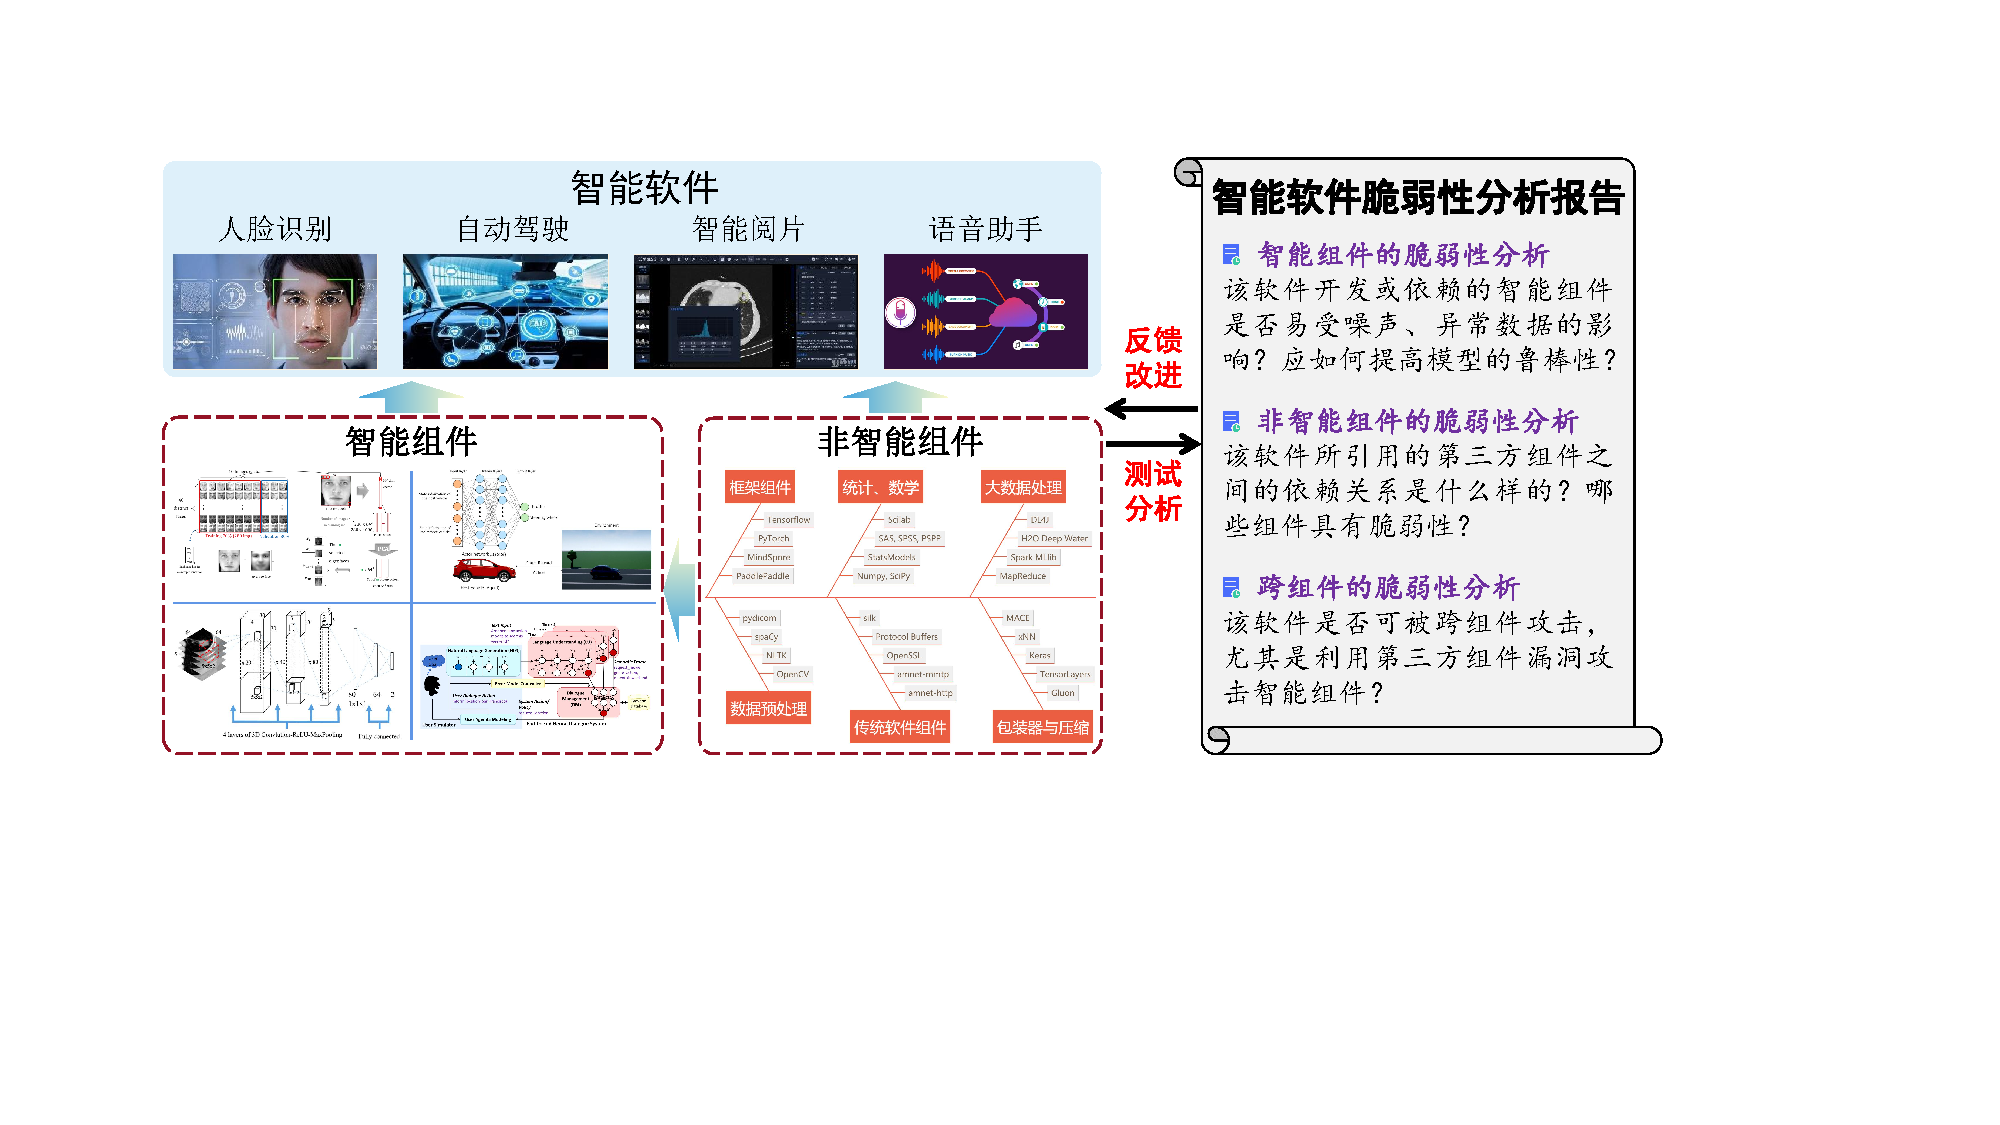
\includegraphics[width=0.98\linewidth]{ch1_AIsoftware.pdf}
    \caption{智能软件依赖于多类型组件,XXX}
    \label{fig:ch1:aisoftware}
\end{figure}


虽然人工智能技术已获得巨大成功,但\textbf{一个可靠的、安全的智能软件系统是其在关
键领域上成功落地的前提}。2018年3月,一辆处在自动驾驶状态的Uber撞击一名女子,致其
不幸身亡,同年7月,Uber宣布停止研发自动驾驶货车。Szegedy等人首次发现,数据中微小
的扰动,即便无法被人类发现,却可能造成智能软件做出错误的判断,进而输出错误的结果
[XX]。由于智能软件越来越多地被部署在自动驾驶、恶意软件检测以及飞机碰撞避免等安全
攸关系统,因此迫切需要找到这些潜在的威胁来提高智能软件的安全性,使之能够应用于更
多关键任务场景。2019年国家新一代人工智能治理专业委员会发布《新一代人工智能治理原
则——发展负责任的人工智能》,该文件中指出“\textbf{人工智能系统应不断提升透明性、
可解释性、可靠性、可控性},逐步实现可审核、可监督、可追溯、可信赖”。

% 2. 现有工作和方法的不足
目前国内外有许多关于人工智能安全性的研究,包括对抗攻击[]、中毒攻击[]、干扰性攻击
[]等。在智能软件测试方面,加拿大阿尔伯塔大学的Lei Ma团队深入研究了深度学习覆盖性
指标[XX]、测试数据生成[XX]、鲁棒性[XX]和模型修复[XX]等方面。国内南京大学的陈振宇
老师团队在对话系统[XX]、医疗[XX]、自动驾驶[XX]、机器翻译[XX]、司法文书[XX]等领域
展开关于智能软件测试方法的深入研究。\textbf{本项目申请人也在自动驾驶软件安全方面
提出了针对神经网络模型的确定性测试数据集生成方法[XX]}。然而,智能软件大量依赖基
础库和第三方依赖库,其脆弱性来源包括智能组件脆弱性、非智能组件脆弱性以及跨组件脆
弱性。\textbf{现有工作主要集中于单个智能/非智能组件的脆弱性,而对多组件之间的交
互影响研究较少,尤其缺乏关于第三方开源组件漏洞对智能组件和基础框架组件脆弱性的影
响}。如\cref{fig:ch1:target}所示,。加个例子。。\textbf{可见,第三方开源组件中存
在的漏洞也可能作为攻击其它组件脆弱点的突破口,从而威胁整个智能软件的安全性}。


% 3. 研究挑战
结合智能软件的特点和安全可靠的应用需求,现有智能软件脆弱性分析具有以下挑战:

\begin{itemize}
    \item[(1)]\textbf{不确定性}:以神经网络模型为代表的智能组件具有不确定性。与
    传统软件不同,智能组件从大规模训练数据中学习对复杂问题的解决规律,容易受噪声
    和异常样本影响,导致做出错误决策。由于输入样本空间较大,难以在真正部署前遍历
    整个输入空间,因此如何对智能组件进行充分性测试是较为重要的挑战。另一方面,由
    于缺乏可解释性,针对智能组件的覆盖性测试难以锁定真正失效原因和脆弱点,导致修
    复较为困难。
    \item[(2)]\textbf{复杂性}:智能软件以大量第三方开源组件为基础,智能组件、基
    础框架组件以及其它第三方组件之间的交互影响尚不明确。一方面,第三方开源组件数
    量极大,版本较多,更新频繁,组件间依赖关系复杂,挖掘可能存在漏洞的脆弱组件难
    度较大。另一方面,第三方组件与智能组件的交互方式尚不明确,其对不同阶段的智能
    组件可能产生的影响不同,智能组件和第三方组件的依赖关系较为复杂。
    \item[(3)]\textbf{高隐蔽性}:智能软件跨组件漏洞具有高隐蔽性。第三方组件漏洞
    给智能软件带来的脆弱点与传统软件不同,利用第三方组件漏洞攻击智能软件不易被发
    现。一方面,利用第三方组件漏洞(如OpenCV CVE-)可以攻击人工智能基础框架中存
    在的漏洞(如XXX),导致智能组件做出错误预测;另一方面,第三方组件漏洞也可以
    直接攻击智能组件,导致智能软件出现中毒攻击、模型萃取、隐私泄露等安全威胁。
\end{itemize}


% 4. 研究方法
本项目直接面向国家人工智能安全可靠发展的重大需求,结合智能软件的特性,从智能组件
确定性、第三方组件脆弱性和跨组件漏洞三个角度研究智能软件的脆弱性,解决了智能软件
不确定性、复杂性和漏洞高隐蔽性带来的挑战,提升智能软件的安全性和可靠性,为智能软
件部署在安全攸关领域提供核心技术支撑。本项目的研究意义主要体现在以下四个方面:

\begin{itemize}
    \item[(1)]\textbf{本项目拟结合神经网络覆盖性测试指标和因果分析,实现具有可解
    释性的智能组件覆盖性测试}。智能组件作为智能软件的核心组成部分,其预测结果影
    响智能软件的正确性。在真正部署智能软件之前,对智能组件进行充分性覆盖测试具有
    重要意义。现有覆盖性测试指标缺乏可解释性,只反映了对特定覆盖条件的满足程度,
    无法定位失效原因。本项目拟结合因果分析和覆盖测试,能够有效分析神经元、参数和
    激活层对测试结果的影响,定位智能组件失效原因,帮助修复智能组件。
    \item[(2)]\textbf{本项目拟构建第三方组件漏洞知识库,以智能组件为输入挖掘非智
    能组件漏洞,实现非智能组件脆弱性测试方法}。涵盖基础框架组件在内的第三方组件
    漏洞,也是造成智能软件脆弱性的重要原因。本项目拟构建面向智能软件的第三方组件
    漏洞知识库,快速有效地发现智能软件里包含的已知组件漏洞;另一方面,为了挖掘智
    能软件中的未知组件漏洞,以智能组件为输入对非智能组件进行模糊测试,发现缓冲区
    溢出、XXX等可能带来安全风险的组件漏洞。
    \item[(3)]\textbf{本项目拟结合单组件脆弱性分析结果和多组件依赖关系,挖掘跨组
    件脆弱通路,实现智能软件跨组件脆弱性分析的通用模型}。智能软件跨组件漏洞具有
    高隐蔽性。第三方组件漏洞给智能软件带来的脆弱点与传统软件不同,利用第三方组件
    漏洞攻击智能软件不易被发现。一方面,利用第三方组件漏洞(如OpenCV CVE-)可以
    攻击人工智能基础框架中存在的漏洞(如XXX),导致智能组件做出错误预测;另一方
    面,第三方组件漏洞也可以直接攻击智能组件,导致智能软件出现中毒攻击、模型萃
    取、隐私泄露等安全威胁。
    \item[(4)]\textbf{本项目拟在基于人工智能的自动驾驶软件上验证上述方案的可行
    性,助力自动驾驶软件安全可靠落地}。近年来,关于自动驾驶软件的安全性和可靠性
    的关注显著增加。截至XXX年。。。本项目拟与XXX和XXX合作,在自动驾驶软件上挖掘
    智能组件、非智能组件以及跨组件的脆弱性,辅助提高自动驾驶软件的安全性和可靠性。
\end{itemize}

% 5. 研究意义

\subsection{国内外研究现状及发展动态分析}\label{relatedwork}

% 根据与本项目的相关性,本节从覆盖充分性指标、神经网络测试数据生成、深度学习框架测试以及第三方组件漏洞挖掘四个方面介绍和分析国内外研究现状。

根据与本项目的相关性,本节从覆盖充分性指标体系、测试数据集生成、测试数据集优选、
深度学习测试可解释性和知识蒸馏技术等五个方面介绍和分析国内外研究现状。

%研究现状:
%1.覆盖充分性指标体系--缺点,找不到失效原因,不可解释
%2.测试数据集生成方法--本项目申请人--缺点,仅仅针对神经网络,也就是智能组件
%3.框架测试方法--缺点,忽略了其它第三方组件漏洞,可以攻击框架漏洞,给智能组件带来安全威胁,也可以直接激活智能组件的脆弱性。
%4.第三方组件漏洞挖掘--缺点,单组建非跨组件,更缺少组件对人工智能模型各阶段的影响分析。



\subsubsection{覆盖充分性指标研究}
针对深度神经网络的结构覆盖测试启发自传统软件的白盒测试。对于传统软件,若测试集遍
历了待测软件所有的语句、分支和路径,则在一定程度上表明测试集对软件的功能进行了充
分性测试~\cite{hilton2018large}。对于深度神经网络而言,其本身的高维连续特性导致
测试集很难遍历所有可能的输入空间,为提高测试集多样性,目前有很多研究提出了关于深
度神经网络的结构覆盖指标,从不同角度测试衡量测试集对模型的覆盖充分
性。\cref{tab:coverage_criteria}总结了现有神经网络测试覆盖指标,其中$m$表示训练
集规模,$n$表示神经元个数,$l$表示\textbf{XXX}。根据覆盖思想的不同,可分为以下六
类:

\begin{table}[htp]
	\renewcommand\arraystretch{1.5}
	\small
	\centering
	\caption{现有神经网络覆盖充分性指标}
	\label{tab:coverage_criteria}
	% \begin{tabular}{p{3cm}p{5cm}p{1cm}p{1cm}p{2cm}}
	\begin{tabular}{ccccc}
		\toprule
		\textbf{序号} & \textbf{主要思想} & \textbf{覆盖指标}       & \textbf{复杂度} & \textbf{文献号}                                                  \\
		\midrule
		1             & 基于单个神经元取值  & 神经元覆盖、$k$-多区间覆盖                    & $O(n)$          & \cite{ma2018deepgauge}\cite{Pei2019DeepXplore} \\
		2             & 训练集神经元边界  & 神经元边界覆盖、强激活覆盖                    & $O(nm)$          & \cite{ma2018deepgauge}                                           \\
		3             & 与训练数据分布的距离  & 意外覆盖,平均偏差等                & $O(nm)$         & \cite{Kim2019Guiding}\cite{Tian2019Testing}            \\
		4             & 神经元激活通路覆盖    & 符号-符号覆盖、距离-符号覆盖等 & $O(nl)$ & \cite{Wang2019DeepPath}\cite{Sun2018Testing} \\
		5             & 神经元的状态转换        & 状态级别覆盖、转换级别覆盖                         & $O(n)$          & \cite{Du2018DeepCruiser}                                         \\
		6             & 神经元组合测试    & $t$-way组合稀疏覆盖、密集覆盖等 & $O(n^2)$ & \cite{ma2019deepct} \\
		\bottomrule
	\end{tabular}
\end{table}





%其中涉及到的覆盖指标主要有神经元覆盖率(NC),$k$区间覆盖率(KMNC),重要性驱动覆盖
%(IDC),神经元边界覆盖率(NBC),强神经元覆盖率(SNC),重要神经元覆盖(INC),意外覆
%盖(SC),神经元激活向量距离(NAVD),平均偏差(MD),重要神经元通路覆盖率(INPC),强
%激活通路覆盖率(SAPC),符号-符号覆盖(SSC),距离-符号覆盖(DSC),符号-值覆盖
%(SVC),距离-值覆盖(DVC),状态级别覆盖(BSC),转换级别覆盖(BTC),$t-way$组合稀疏
%%%%覆盖($t-way$ CSC),$t-way$组合密集覆盖($t-way$
%CDC),$(p,t)$完整性覆盖($(p,t)$ C)等指标。

%DeepXplore~\cite{Pei2019DeepXplore}、DeepGauge~\citess{ma2018deepgauge}、IDC~\citess{Gerasimou2020Importance}
%等工作主要围绕神经元覆盖率、K区间覆盖率、重要性驱动覆盖等测试覆盖指标。

\begin{itemize}
	\item \textbf{基于单个神经元取值},受结构覆盖思想启发,部分研究者提出度量神
	      经元被覆盖的程度来评估测试充分性。Pei等人~\cite{Pei2019DeepXplore}首次
	      提出了针对深度学习模型白盒测试指标,即神经元覆盖,将取值高于阈值的神经
	      元视为被激活,并计算被激活神经元的比例。 Ma等人~\cite{ma2018deepgauge}
	      提出了$k$-多区间覆盖指标,基于每个神经元在训练集上的取值范围,将其划分
	      为多个取值区间,并计算对神经元值区间的覆盖率。
	      %Gerasimou等人~\citess{Gerasimou2020Importance}设计了通过衡量神经元对分类结果的影响比例提出了重要性驱动覆盖标准。

	\item \textbf{基于训练集神经元的值边界},Ma等人~\cite{ma2018deepgauge}提出神
	经元边界覆盖指标和强激活覆盖指标,计算测试集中神经元的值超过训练集的上下边界
	的比例。

	\item \textbf{基于神经元激活值分布},Kim等人~\cite{Kim2019Guiding}提出了“意
	      外”覆盖指标,衡量模型在测试集和训练集中神经元数据分布距离。Tian等人
	      ~\cite{Tian2019Testing}提出白盒测试框架DeepInspect来检测深度神经网络中
	      的混淆和偏差错误。

	\item \textbf{基于神经元激活通路},Wang 等人~\cite{Wang2019DeepPath}提出了一
	      组针对神经网络模型的路径驱动的测试度量指标,能够更好地识别对抗性样本。
	      Sun等人~\cite{Sun2018Testing}提出将传统的MC/DC覆盖标准应用于深度神经网
	      络,并在此基础上采用梯度搜索的方法生成新的测试集。

	\item \textbf{基于神经元状态},Du等人~\cite{Du2018DeepCruiser}针对循环神经网
	      络提出了状态级别和转换级别两种测试覆盖指标,根据覆盖范围反馈生成具有高
	      覆盖率的测试集,并对基于循环神经网络的自动语音识别系统进行检测。

	\item \textbf{基于神经元组合分布},Ma等人~\cite{ma2019deepct}将组合测试应用
	于神经网络,提出了$t$-way组合稀疏覆盖、$t$-way组合密集覆盖和$(p,t)$完整性覆
	盖等指标。
\end{itemize}

测试覆盖指标是衡量测试集对深度学习模型测试充分性的标尺,是深度学习测试
的重要研究问题之一。{\kaishu 现有测试覆盖指标主要聚焦于对神经网络模型的神经元结构的覆盖研
究,缺少对高层次语义表示覆盖的研究,因此缺乏可解释性。另一方面,现有指标伸缩性较
差,其计算时间和指标有效性难以应对实际大规模模型。本项目拟提出基于知识萃取的可解
释测试覆盖指标,将知识蒸馏和知识回顾应用于神经网络模型测试,从而提升测试指标的伸
缩性和可解释性。}


\subsubsection{测试数据生成方法}

为提高深度学习模型的可靠性,使用足够的测试输入对其一般行为和各种边界条件下的行为
进行充分测试是十分必要的。在对深度学习模型的测试中,如何生成更具代表性的和更容易
暴露模型错误行为的测试数据已成为深度学习测试的一个研究重点。如
\cref{tab:testingDataGen}所示,现有测试数据生成方法可分为以下三类:

\begin{table}[htp]
	\renewcommand\arraystretch{1.5}
	\small
	\centering
	\caption{深度学习模型测试数据生成方法总结}
	\label{tab:testingDataGen}
	% \begin{tabular}{cp{5cm}p{2cm}cp{2cm}}
	\begin{tabular}{cccccc}
		\toprule
		\textbf{序号} & \textbf{算法思想} & \textbf{评价方法}               & \textbf{测试数据} & \textbf{文献号}             \\
		\midrule
		1             & 模糊测试          & 测试覆盖率、效率 & 图像、文本 & \cite{Odena2019TensorFuzz}\cite{Guo2018DLFuzz}\cite{xie2019coverage} \\
		2             & 符号执行          & 测试覆盖率、像素重要性等                              & 图像、代码              & \cite{Gopinath2018Symbolic}\cite{Sun2018Concolic} \\
		3             & 对抗样本          & 准确率、失真度、人类对比评价等 & 图像 & \cite{Xiao2018Spatially}\cite{Wicker2018FeatureGuided}\cite{He2018Decision} \\
		\bottomrule
	\end{tabular}
\end{table}


\begin{itemize}
	\item \textbf{基于模糊测试的思想},通过随机或者特定规则将种子输入进行变换,
	生成新的测试数据,观察模型在边界条件下是否会发生错误。Guo等人
	~\cite{Guo2018DLFuzz}首次提出神经网络模糊测试框架DLFuzz,用于指导生成暴露模
	型错误行为的测试数据。Odena等人~\cite{Odena2019TensorFuzz}利用测试覆盖指标指
	导模糊测试。在此基础上,Xie等人~\cite{xie2019coverage}提出了一个自动化模糊测
	试框架DeepHunter,使用6种测试覆盖指标实现了在深度学习模型开发和部署两个阶段
	的自动化测试。

	\item \textbf{基于符号执行},Sun等人~\cite{Sun2018Concolic}在测试覆盖指标的
	基础上提出了DeepConcolic,结合具体执行和符号分析,提高神经网络的测试覆盖
	率。Gopinath等人~\cite{Gopinath2018Symbolic}提出了一种轻量级符号执行技术并将
	其应用于图像分类算法的测试,以解决重要像素的识别以及创建1像素和2像素攻击等关
	键问题。

	\item \textbf{基于对抗样本的方法},通过向原始样本添加微小扰动的方式产生对抗
	      样本,使深度学习模型做出错误预测。在白盒攻击方面,Xiao等人
	      ~\cite{Xiao2018Spatially}提出了基于空间变换的图像对抗样本生成方法。He
	      等人~\cite{He2018Decision}提出了一种针对区域分类的对抗样本生成方法。在
	      黑盒攻击方面,Wicker等人~\cite{Wicker2018FeatureGuided}提出一种特征引
	      导的鲁棒性测试方法,通过双方博弈游戏的方式确定特征和操作像素点,并利用
	      蒙特卡罗树搜索算法逐步探索博弈状态空间来生成对抗性样本。
\end{itemize}


在深度学习模型部署前找到容易导致模型错误行为的输入数据是必要的。现有测试数据生成
方法主要分为两类:一类受传统软件测试方法启发,在输入种子数据的基础上允许在语义大
致不变的前提下对输入进行变异,以提高覆盖率为导向生成新数据;另一类基于对抗样本,
通过基于梯度等方法搜索导致模型错误预测的最小扰动,生成新测试数据。{\kaishu 然
而,由于神经网络的黑盒特性,这两类测试数据生成方法虽然能够暴露模型错误行为,但测
试结果缺乏可解释性,测试人员很难掌握测试成功或失效的原因,因此除扩充训练集外,对
模型修复的作用较少。本项目拟提出具有可解释性的深度学习模型测试框架,从模型和测试
数据两个角度提高深度学习测试的可解释性。}













\subsubsection{测试数据选择方法}

由于深度学习模型的输入数据的样本空间通常较大,而人工标注测试预言的成本较高,因此
很难在系统部署前检测每个潜在数据样本的预测正确性。为解决这个问题,部分研究提出测
试数据选择方法,从大规模无标注数据中选择出优先标注和测试的输入数
据。\cref{tab:testingDataPri}总结了现有测试数据选择方法,根据选择思想的不同可分
为以下三类:

\begin{table}[htp]
	\renewcommand\arraystretch{1.5}
	\small
	\centering
	\caption{深度学习模型测试数据集优选方法总结}
	\label{tab:testingDataPri}
	\begin{tabular}{cccc}
		\toprule
		\textbf{序号} & \textbf{算法思想}  & \textbf{测试对象} & \textbf{文献号}                                                    \\
		\midrule
		1             & 采用变异测试的思想       & 图像              & \cite{Wang2021Prioritizing}\cite{Ma2018DeepMutation}  \cite{Liu2022DeepState}                    \\
		2             & 基于测试数据的执行结果       & 图像、自然语言  & \cite{Byun2019Input}\cite{Shen2020MultipleBoundary}\cite{Feng2020DeepGini}\cite{Hu2022AnEmpirical}\cite{Gao2022Adaptive} \\
		\bottomrule
	\end{tabular}
\end{table}

\begin{itemize}

	\item \textbf{基于变异测试的思想},部分研究对神经网络模型进行变异,优选能够
	      检测出较多变异模型的测试数据进行标注。Ma等人
	      ~\citess{Ma2018DeepMutation}从训练数据、训练代码和深度学习模型三个角度
	      注入错误,通过错误检出率衡量测试数据质量。Wang等人
	      ~\citess{Wang2021Prioritizing}利用learning-to-rank算法
	      ~\citess{liu2019exploiting}构建测试数据排序模型,能够针对不同的深度学
	      习模型自动优选具有较高错误检测能力的测试数据。Liu等人
	      ~\citess{Liu2022DeepState}提出一种针对循环神经网络的测试集优选方法
	      DeepState,通过捕获神经元状态的变化来识别可能预测错误的测试数据。  

	\item \textbf{基于测试数据的执行结果}, Byun等人~\citess{Byun2019Input}从置
	      信度、不确定性和意外度等三个指标衡量测试数据的错误检测能力,并评估测试
	      数据对于模型再训练的提升。Feng等人~\citess{Feng2020DeepGini}提出一种基
	      于数据统计的测试集优选方法DeepGini,通过输出概率分布识别可能被错误分类
	      的测试数据。Shen等人~\citess{Shen2020MultipleBoundary}将测试数据聚类到
	      深度学习模型的多个边界区域中,从边界区域中均匀选择样本以确保每个边界都
	      有足够的测试数据。Hu等人~\citess{Hu2022AnEmpirical}提出了面向测试集优
	      选的数据分布敏感指标,用来减轻数据分布差异对标注数据集选择的影响。

\end{itemize}

{\kaishu 现有针对深度学习模型的测试数据集优选方法,主要集中于测试数据是否能够反
映模型错误行为,而对测试数据导致模型错误的原因缺乏研究。本项目拟提出基于反馈偏置
的自适应测试集生成,在可解释测试覆盖度量的基础上,选取代表性的样本来解释模型结
果,估算模型性能;同时,自适应找到导致模型错误行为的测试数据优先标注,提高测试集效率。}










\subsubsection{深度学习测试可解释性}

\iffalse
	Zhang等人~\citess{zhang2021duo}提出了一种结合模糊测试和差分生成输入的深度学习框架测试方法Duo,用于解释和评估TensorFlow、PyTorch、MNN、MXNet等深度学习框架;也提出了一种基于模糊测试的算子级精度测试方法Predoo~\citess{zhang2021predoo},用于估计TensorFlow中单个深度学习算子的精度误差。
	Hu等人~\citess{Hu2019DeepMutationPlusPlus}提出了一种基于变异测试的DNN工具DeepMutation++,用于对包括前馈神经网络(FNN)和有状态循环神经网络(RNN)在内的DNN的质量评估,不仅可以静态分析DNN模型对整个输入的鲁棒性,还可以通过运行时分析识别顺序输入的易受攻击部分。
	Xie等人~\citess{Xie2019DiffChaser}提出了一种自动黑盒测试框架DiffChaser,用于检测深度学习模型在量化、压缩前后的非目标或目标不一致性。
	Du等人~\citess{Du2020Marble}提出了的方法Marble构建了一个概率模型,通过抽象来紧凑表征RNN的鲁棒性,用于对基于RNN的深度学习系统进行定量的鲁棒性分析。

	Luo等人~\citess{luo2021graph}将算子级别的覆盖指标引入图论,提出了一种基于图的模糊测试方法来捕捉深度学习框架异常、提高深度学习框架质量和可解释性的方法。
	Du等人~\citess{Du2019DeepStellar}~\citess{Du2019AQuantitative}提出了一个基于对抗性样本检测和覆盖引导测试生成的深度学习模型测试方法DeepStellar,基于两个轨迹相似性指标和五个覆盖充分性指标对循环神经网络(RNN)进行定量分析和可解释性研究。
	Lee等人~\citess{Lee2020Effective}提出了一种对神经网络进行白盒测试的新方法Adapt,通过使神经元选择策略不断地自适应正在进行的测试状态,增强了深度神经网络的可解释性,在覆盖率和对抗性输入方面有有效表现。
	Wang等人~\citess{wang2020deepsonar}提出一种识别AI合成假声音的方法DeepSonar,利用对分层神经元激活模式学习来增强深度神经网络在语音识别方面的可解释性,推测真实和AI合成的假声音之间的细微差异,同时也对操纵攻击(例如语音转换和附加现实世界噪声)的情况具有鲁棒性。
\fi



由于深度学习模型的黑盒特性,开发人员很难将测试结果与模型行为联系起来,深度学习测
试能够提供的有效修复信息较少。目前关于可解释性的研究工作主要集中于深度学习模型本
身的可解释性,而对测试结果的可解释性研究较少。Xie等人~\citess{Xie2021NPC}提出了
神经元路径覆盖指标,类似于传统的程序控制流图,首先从深度神经网络中提取决策图用来
表示模型的决策逻辑,然后基于决策图的控制流和数据流,该方法提出了两种路径覆盖的变
体来衡量测试数据在执行决策逻辑时的充分性。该测试方法在一定程度上反映出模型的决策
逻辑,但由于模型本身缺乏可解释性,难以从控制流或数据流路径上辅助开发人员找到模型
失效的原因,从而帮助修复模型。此外,Chen等人~\citess{Chen2020Practical}提出了一
种可解释的测试数据选择方法,利用基于实例的可解释算法MMD-critic选取具代表性的测试
输入来估算模型在整个测试集上的准确性。该方法的可解释性主要体现在测试数据的选择流
程上,而对测试反馈的可解释性仍然不足。

{\kaishu 虽然结构覆盖测试能够在一定程度上提高测试集的充分性,但由于模型本身的黑
盒特性,现有的深度学习模型测试工作也缺乏可解释性,开发人员很难建立测试结果与模型
行为之间的联系。本项目拟提出针对深度学习模型的可解释测试框架,采用知识蒸馏和知识
回顾的思想,从白盒和黑盒两个角度分别提出可解释测试覆盖指标,通过测试反馈辅助开发
人员修复模型。}

%然而在现实情形中,智能软件大量依赖基础库和第三方依赖库,其脆弱性来源包括智能组件脆弱性、非智能组件脆弱性以及跨组件脆弱性,而智能组件、基础框架组件以及其它第三方组件之间的交互影响尚不明确,第三方开源组件数量极大,版本较多,更新频繁,组件间依赖关系复杂,挖掘可能存在漏洞的脆弱组件难度较大。



\subsubsection{知识蒸馏技术}

知识蒸馏是指一种教师-学生(Teacher-Student)模型训练结构,其目标是以尽可能小的代
价将教师模型学到的知识迁移到简单的学生模型中~\citess{Gou2021KnowledgeDA}。该技术
被广泛应用于模型压缩,目前在图像、文本、音频等多种模态数据的处理任务中均有应用。
在计算机视觉方面,Hou等人~\citess{Hou2020CVPR}通过传输图像样本中不同区域之间的结
构关系,将教师网络学习到的场景结构知识迁移给学生执行道路标记分割任务。Fu等人
~\citess{Fu2020Ultrafast}提出将教师模型学习到的空间和时间知识迁移到低分辨率的轻
量级时空网络中来执行视频注意预测任务,高分辨率数据上训练得到的知识在低分辨率图片
处理任务上具有重要价值,同时能够降低对于计算机资源和存储的要求。在自然语言处理方
面,Wang等人~\citess{Wang2020StructureLevelKD}和Mukherjee等人
~\citess{Mukherjee2020XtremeDistilMD}将若干单语言的教师模型学习到的结构知识和内
部特征迁移到统一的多语言学生模型,来得到轻量级的多语言序列标注模型,而且其性能表
现比原有复杂模型更优。在语音识别领域,Aguilar等人
~\citess{Aguilar2020KnowledgeDF}提出将教师网络的多个Transformer层的特征知识压缩
到学生的单个Transformer层中,Liu等人~\citess{Liu2019EndtoEndST}提出引入自适应层
来压缩Transformer结构,在保持transformer对长序列学习问题的优越性的同时,也减轻了
它过大的参数规模,便于计算和存储。

部分研究将知识蒸馏用于生成具有可解释性的学生模型。Liu等人
~\citess{Liu2018ImprovingTI}将深度神经网络提炼并表示成决策树,将已有问题转化为多
输出回归问题,可以同时获得良好的性能和可解释性。另一方面,知识蒸馏本身也具有一定
的可解释性,从而可以帮助生成可解释的轻量级模型。 Cheng等人
~\citess{Cheng2020ExplainingKD}通过对深度神经网络中间层的量化和分析,提出了对知
识蒸馏所得学生模型性能优越的解释,认为知识蒸馏能够学习到更多的视觉概念。此
外,Phuong等人~\citess{Phuong2019TowardsUK}通过研究线性和深度线性分类器,提出了
蒸馏成功的三个关键原因:一是数据分布的几何特性,二是优化偏差,梯度下降优化找到对
蒸馏目标的非常有利的极小值,三是强单调性,即当训练集的大小增加时,学生分类器的预
期风险总是降低。


{\kaishu 目前知识蒸馏技术已被广泛应用于模型压缩,本项目拟利用部分知识蒸馏技术对
深度学习模型可解释性的提升,融合Kolmogorov-Smirnov检验、D检验等方法构建具有可解
释性的测试覆盖指标,总结归纳模型错误行为的原因,指导训练数据集扩充和模型优化。}








% 因为写 demo,我把参考文献放这里了,真写本子的时候,还是要放在国内外概况那边
\begin{spacing}{1.3} % 行距
	\zihao{5} \songti
	\bibliographystyle{gbt7714-nsfc}
	\bibliography{ref,cai_refs}
	\vspace{11bp}
\end{spacing}


\NsfcSection{2}{项目的研究内容、研究目标,以及拟解决的关键科学问题}{(此部分为重
点阐述内容);}

\subsection{研究内容}\label{ch2content}

本项目面向医疗卫生行业的数据分析需求,针对电子医疗记录分析存在的研究队列识别困
难、记录时间不规则、模型解释匮乏等问题,以深度学习为基础手段,研究电子医疗记录分
析建模的理论和方法,力争构建端到端的电子医疗记录分析方案,突破队列识别、EMR插补
和可解释性分析模型等关键技术,并在基于电子医疗记录的临床任务上验证本项目的研究成
果。

项目研究工作从队列识别、EMR插补、可解释分析模型和临床任务验证四个层次展开,本项
目的挑战、科学问题和研究内容关系如图~\ref{fig:ch2:rc}所示。各部分研究内容具体介
绍如下:

\begin{figure}[htp]
    \begin{small}
        \begin{center}
            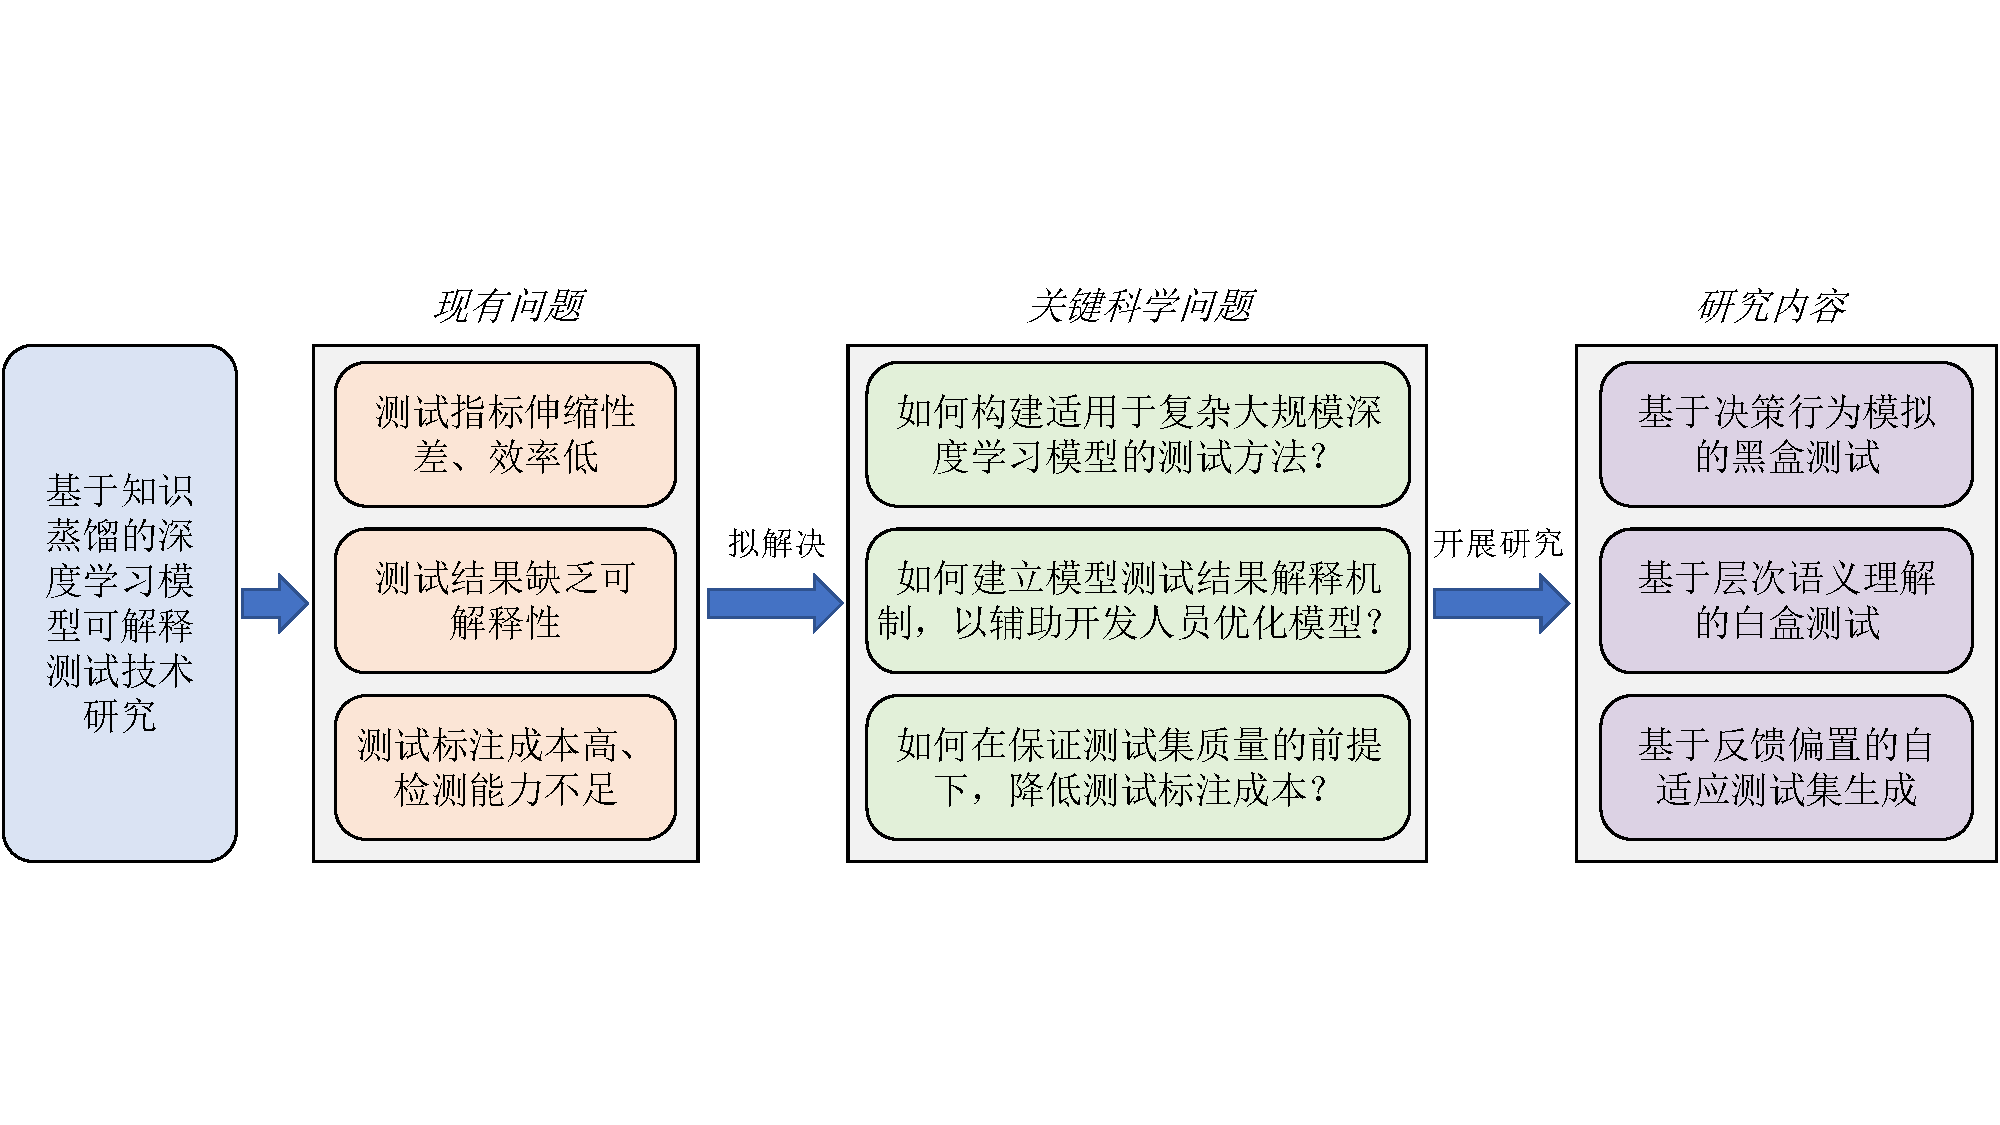
\includegraphics[width=0.95\textwidth]{ch2_framework.pdf}
        \end{center}
        \caption{挑战、科学问题和研究内容关系图}
        \label{fig:ch2:rc}
    \end{small}
\end{figure}

\subsubsection{基于决策行为模拟的黑盒测试}

借鉴传统软件的路径覆盖测试方法,许多研究提出针对深度学习模型的覆盖性测试方法(参
见\ref{relatedwork} 国内外研究现状及发展动态分析),这些测试覆盖指标和方法主要是
针对白盒的场景,即测试者掌握所有的训练数据和整个深度学习模型,\textbf{但在许多场
景中,测试者无法访问训练数据和模型内部结构,但仍需要对模型的泛化能力进行测试,即
黑盒测试,如深度学习模型是某个公司私有的或者由第三方机构提供,他们只提供了接口或
者打包的可执行程序。}因此,本项目面向黑盒测试场景,研究基于决策行为模拟的黑盒测
试方法。

以分类模型为例,给定一个黑盒深度学习模型$\mathcal M$和测试数据集$\mathcal
D_{\text{test}}=\{x^{(i)},y^{(i)}\}$,测试者可以得到模型针对每个输入
$x^{(i)}$(input)的输出$\hat{y}^{(i)}$,通常是该输入属于各个类别的概率分布,除
此之外,测试者无法知道该模型的训练数据和内部结构。可见,深度学习模型黑盒测试面临
两个主要问题:
\begin{itemize}
    \item \textbf{如何建立模型有关的测试方法?}仅有的几个黑盒模型测试方法仅针对
    数据的多样性进行评估,无法准确反映模型的性能,也不能给模型改进提供有效建议。
    \item \textbf{如何掌握模型的决策机制?}黑盒测试中,测试者无法了解模型的结
    构,模型对测试用例的决策过程无法知晓。
\end{itemize}

\begin{figure}[htp]
    \begin{small}
        \begin{center}
            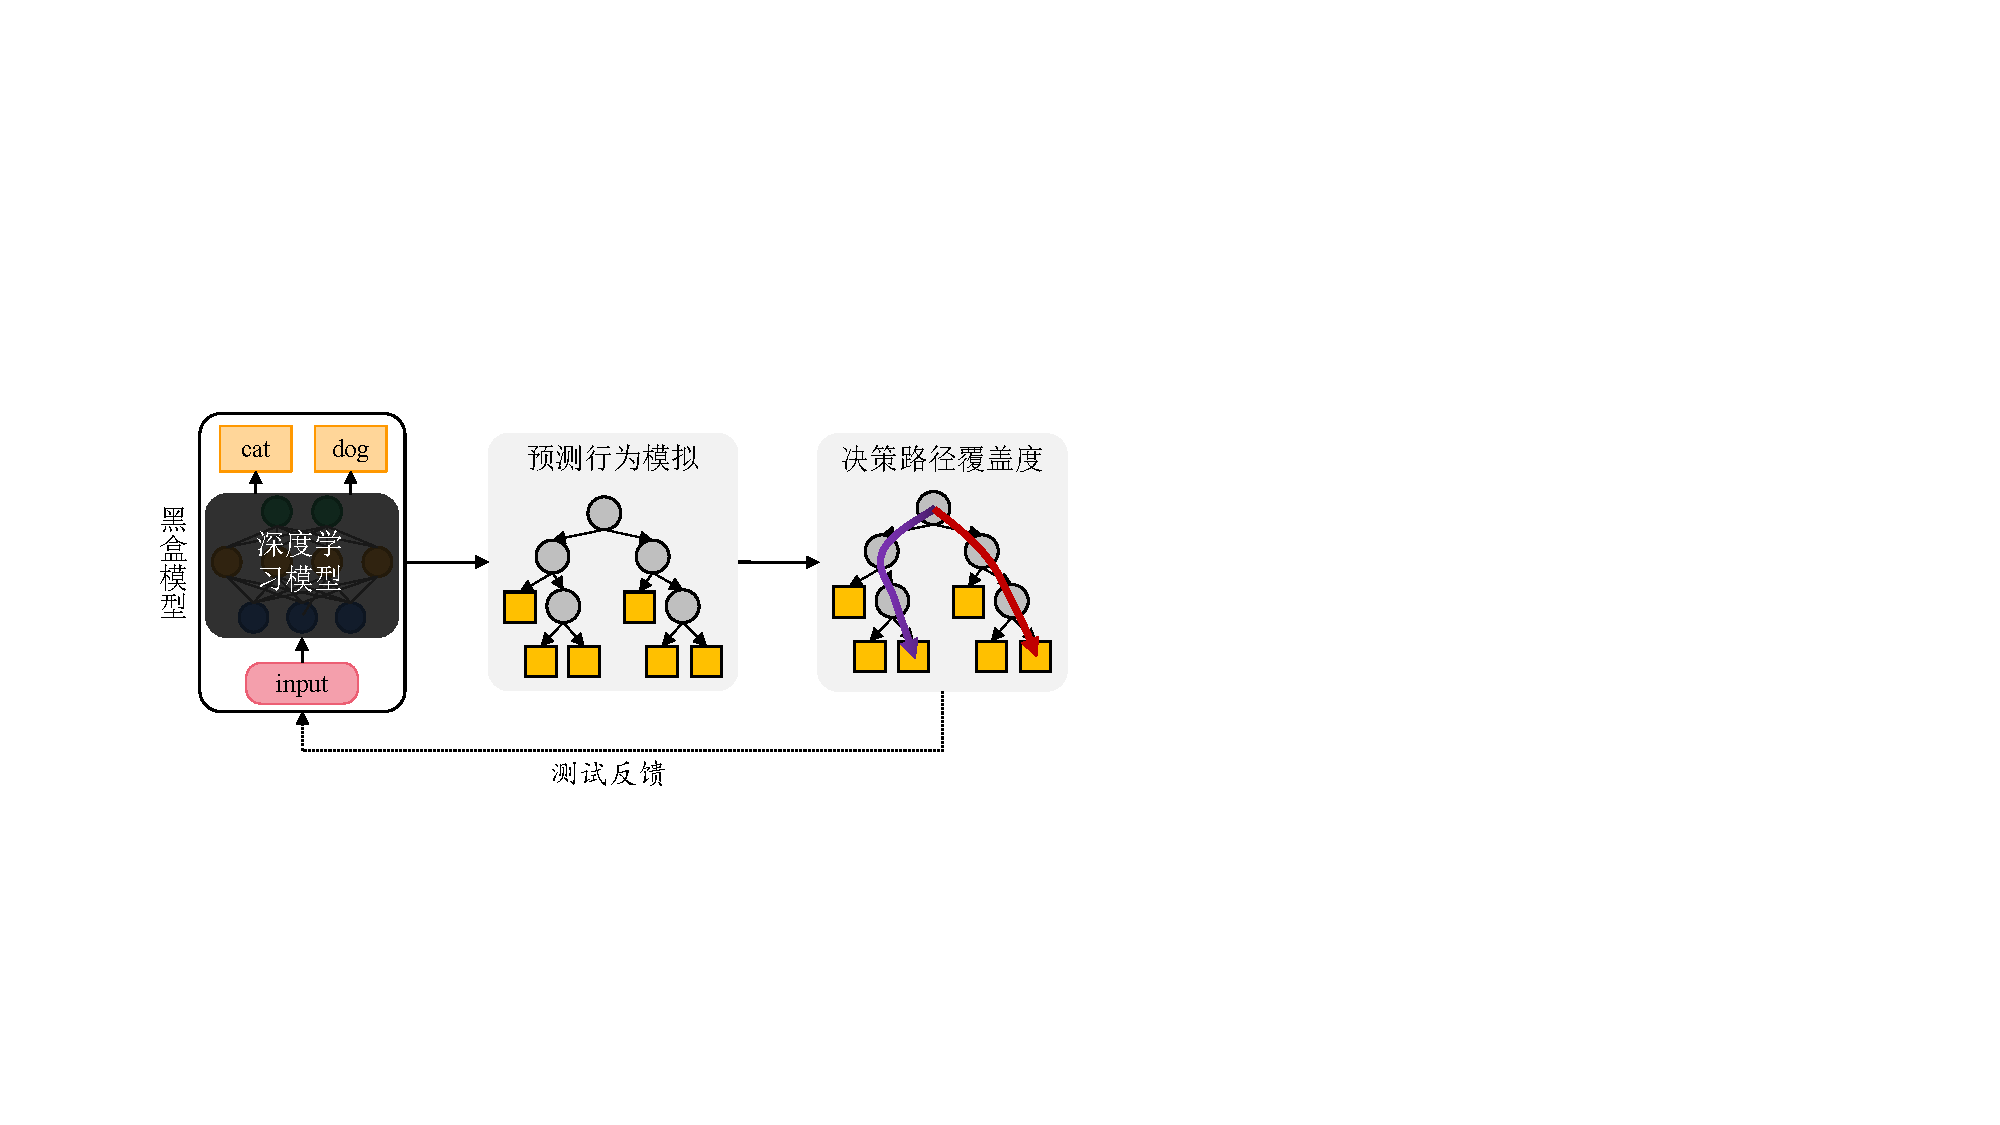
\includegraphics[width=0.75\textwidth]{ch2_2Btest.pdf}
        \end{center}
        \caption{基于决策行为模拟的黑盒测试研究内容}
        \label{fig:ch2:2Btest}
    \end{small}
\end{figure}
本项目深度学习模型黑盒测试的主要研究内容如\cref{fig:ch2:2Btest}所示,\textbf{本项目首先
研究针对黑盒模型的预测行为模拟方法,拟利用知识萃取的方法,通过建立副本模型
$\mathcal M^\prime$(如决策树)萃取黑盒模型$\mathcal M$的知识,模拟$\mathcal M$
的预测行为;然后,在副本模型的基础上,本项目拟建立基于决策路径覆盖度的测试方法,
通过覆盖度指标反映模型的决策机制和泛化能力。}

\subsubsection{基于层次语义理解的白盒测试}

除了黑盒测试的场景,白盒测试的需求也非常多,如企业自己开发的深度学习模型,在白盒
测试中,测试者可以访问模型的内部结构$\mathcal M(\bm W, \bm b)$和训练数据集
$\mathcal D_{train}=\{(x^{(i)}, y^{(i)}\})$。目前,针对深度学习模型的白盒测试方
法可扩展性和可解释性较差,无法应用于大规模深度学习模型,如
BERT~\cite{kenton2019bert},MAE~\cite{he2021masked}等,而且测试结果无法给模型训
练提供有效反馈,辅助模型优化。因此,\textbf{本项目提出针对白盒深度学习模型的层次
语义理解方法,并利用各层的决策语义训练一个副本模型中,保证副本模型的决策路径与原
白盒模型一致;然后围绕副本模型进行决策路径覆盖度测试,决策路径具有较强的可解释
性,可引导测试数据生成和模型优化。}

\begin{figure}[htp]
    \begin{small}
        \begin{center}
            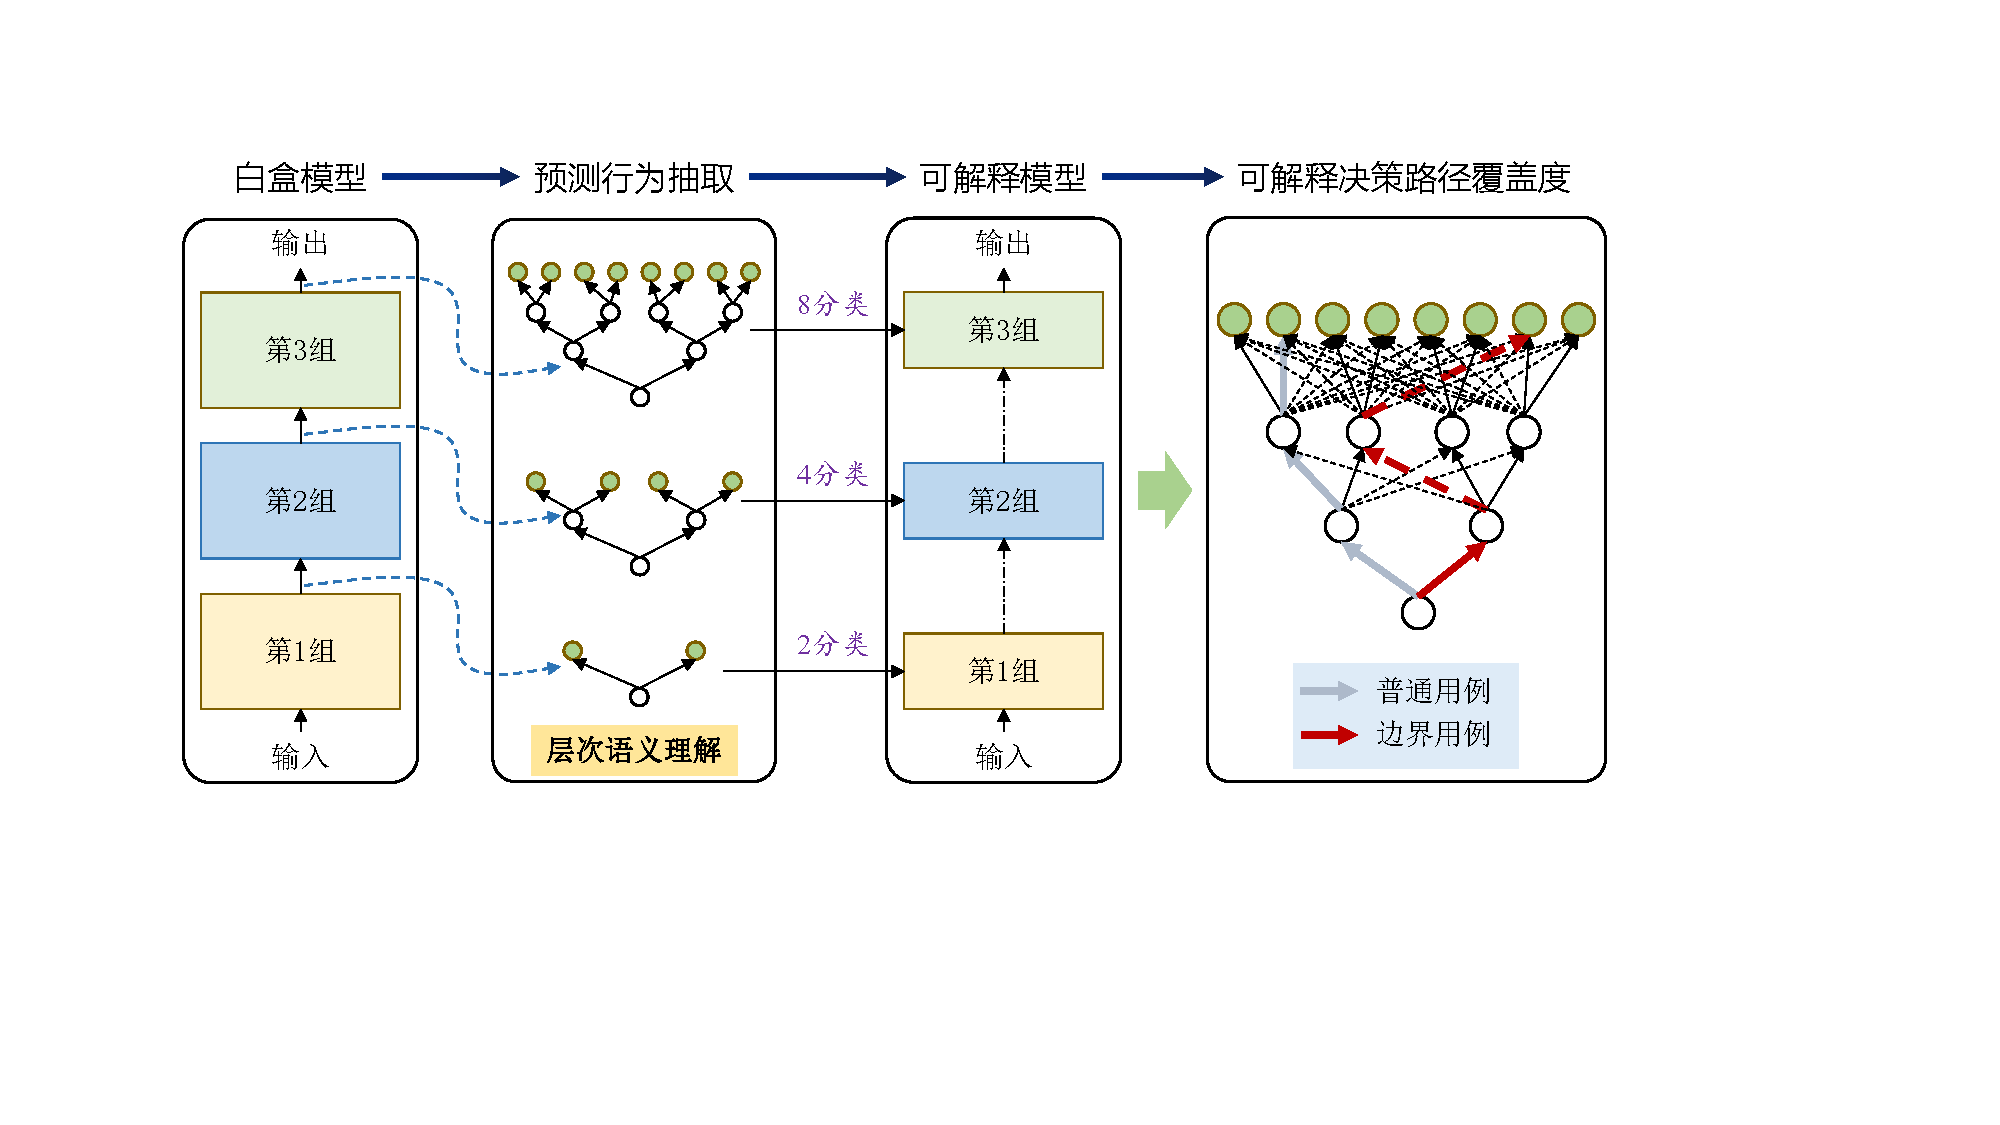
\includegraphics[width=0.9\textwidth]{ch2_WBtest.pdf}
        \end{center}
        \caption{基于层次语义理解的白盒测试研究内容}
        \label{fig:ch2:WBtest}
    \end{small}
\end{figure}

本项目基于层次语义理解的白盒测试研究内容如\cref{fig:ch2:WBtest}所示,在白盒测试
的场景下,本项目首先研究如何从深度学习模型中抽取出各层(layer)的决策语义信息,
研究表明,深度学习模型对输入的决策是由粗粒度到细粒度的。\cref{fig:ch2:WBtest}举
例说明了从3组神经网络层的输出抽取各组网络的预测行为,例如:输入一个猫的图片,第1
组神经网络判断该图片是否是动物,接着,第2组神经网络判断该图片是否是猫科动物,最
后,第3组神经网络将该图片分类为猫。\textbf{本项目拟研究如何实现层次语义理解,自
动地从深度学习模型中抽取出各层的决策语义}。

在层次语义理解的基础上,\textbf{本项目拟融合白盒模型的多层次决策语义训练一个副本
模型,使该副本模型的决策路径与原白盒模型一致,且具有良好的可解释性}。此外,知识
蒸馏得到的模型通常规模较小,和直接测试原白盒模型相比,测试副本模型可有效提高测试
效率。\textbf{在得到可解释的副本模型后,本项目拟研究并提出针对该可解释模型的决策
路径覆盖度,用于分析测试样本的多样性和充分性}。

\subsubsection{融合反馈偏置的自适应测试集生成}
深度学习模型的测试依赖于有标签的测试集,以判断模型预测结果是否符合预期,然而,测
试集的标注成本通常较高。一方面,深度学习模型的测试输入标注通常依赖于人工经验,一
个测试数据需要多个经验丰富的标注人员来标出,以保证标注正确性;另一方面,为了测试
充分性和准确评估模型性能,测试集的规模通常较大,尽可能代表真实的测试数据分布,导
致标注成本较高。因此,{需要合理平衡测试集的规模和质量,在有限标注成本空间内选取
对样本空间具有高代表性的测试数据,生成规模相对较小的高质量测试集优先标注}。\textbf{本项
目拟提出一种可解释的自适应测试集生成方法,给定输入空间内大规模无标注测试数据,针
对充分性测试和模型性能评估两个测试目标,结合测试执行反馈,筛选出具有不同检测能力
的测试数据,生成指定规模的高质量测试集。}

\begin{figure}[htp]
    \begin{small}
        \begin{center}
            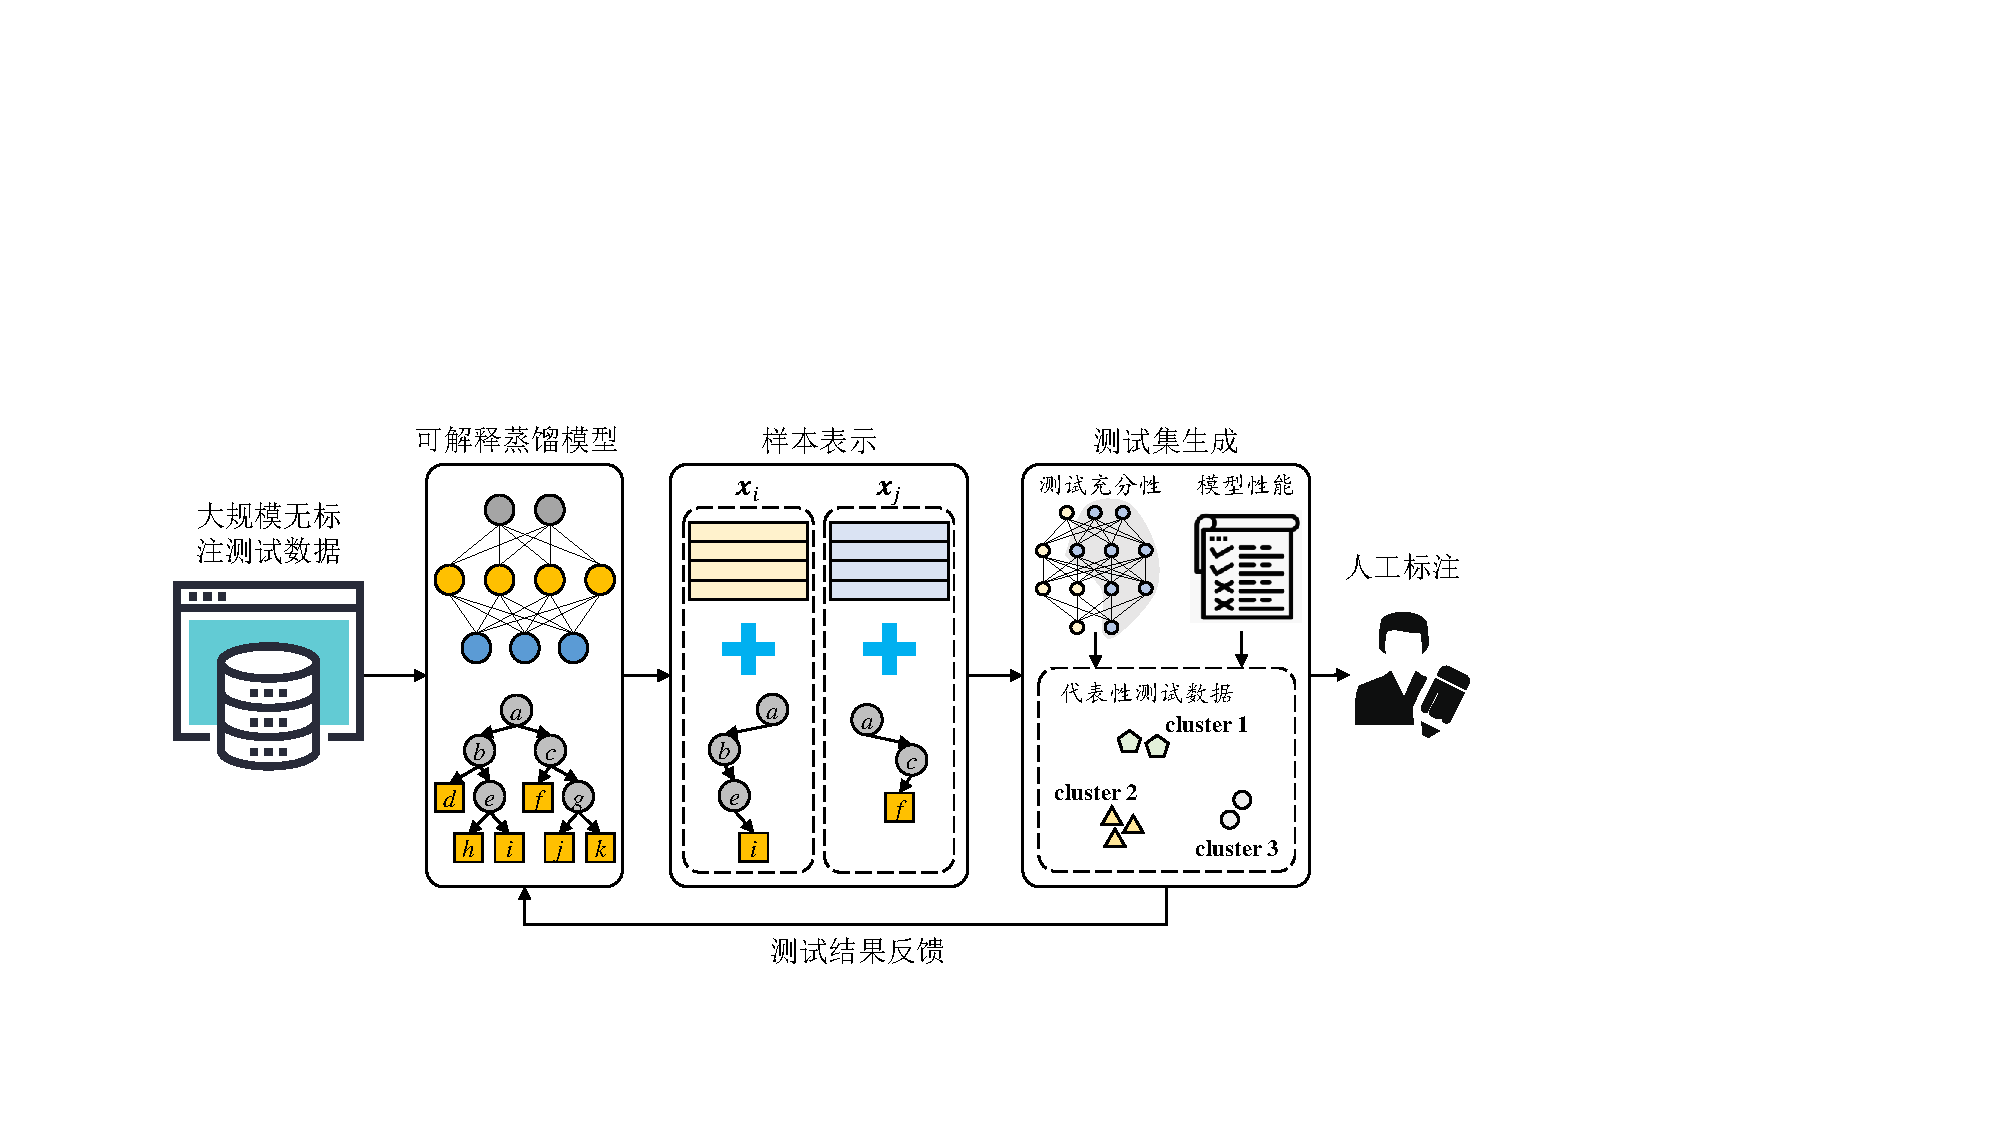
\includegraphics[width=0.95\textwidth]{ch2_TestSelection.pdf}
        \end{center}
        \caption{可解释预测模型研究内容}
        \label{fig:ch2:testselection}
    \end{small}
\end{figure}

如\cref{fig:ch2:testselection}所示,本项目拟在自适应测试中考虑可解释性,现有工作
缺乏对测试数据生成和测试结果反馈的可解释性,导致针对深度学习的有效测试信息较少,
难以辅助修复模型缺陷。结合前面研究内容,本项目可从黑盒和白盒两个角度将复杂神经网
络抽象为可解释蒸馏模型,对每个输入数据都输出具有可解释性的决策路径。针对给定大规
模无标注测试数据,可经过可解释蒸馏模型得到所有测试数据的决策路径分布,具有相同决
策路径的测试数据为一组。根据每组测试数据规模大小,采用聚类分析将具有相同决策路径
的测试数据分为多个类簇,利用基于最大平均差异法为从每簇测试数据中选取固定总数的测
试数据作为代表性数据,得到与无标注数据集有近似决策路径分布的初始子集。\textbf{本
项目拟从充分性测试和准确评估模型两个测试目标来制定自适应反馈机制,将复杂神经网络
抽象成可解释蒸馏模型,选取与大规模无标注测试数据具有近似决策路径分布的代表性数据
进行标注,为测试人员提供全阶段的可解释测试方法}。


\subsection{研究目标}\label{ch2target}

本项目从深度学习模型部署的实际需求和人工智能软件安全性的前沿问题出发,针对深度学
习模型测试方法伸缩性差、缺乏可解释性和测试数据标注成本高等问题,分别建立基于决策
路径的黑盒测试和白盒测试方法,在此基础上构建融合反馈偏置的自适应测试集生成方法,
形成一套从测试指标、测试用例生成到测试反馈的深度学习可解释测试解决方案,并在自动
驾驶、人脸识别等实际应用中检验研究成果的效果。

具体研究目标包括:

\textbf{在技术方面},本项目拟在以下三方面实现技术突破: (a) 提出基于决策行为模拟
的黑盒测试方法,利用知识蒸馏技术,训练副本模型,模拟黑盒模型的预测行为,实现伸缩
性强、可解释性的黑盒测试;(b) 提出基于层次语义理解理解的白盒测试方法,抽取模型的
中间表示和决策路径,训练副本模型,实现伸缩性强、可解释的白盒测试;(c) 提出融合反
馈偏置的自适应测试集生成方法,针对测试目标,结合测试执行反馈,选取与大规模无标注
测试数据具有近似决策路径分布的代表性数据。

\textbf{在成果形式方面},本项目力争在CCF-A类推荐期刊/会议或其他SCI期刊上发表高水
平论文3-6篇;申请专利2项;并开源相关研究工作,供用户下载,并提供说明和使用文档。

\textbf{在人才培养方面},通过本项目研究,培养深度学习测试、人工智能安全等前沿领
域的青年人才,拟培养研究生2-3人。

\subsection{拟解决的关键科学问题}

基于上述研究目标和研究内容,本项目拟在以下几个关键理论和技术问题上有所突破:

\subsubsection{在黑盒场景下,仅根据模型输入输出,模拟构建黑盒模型的决策路径}

在黑盒测试中,测试者无法了解待测模型的内部结构和训练数据集,仅能得到测试输入输
出,因此无法知晓模型对输入样本是如何决策判断的。现有测试覆盖指标主要基于神经网络
结构的覆盖,仅有黑盒测试研究局限于与模型无关的测试数据多样性的评估,尚未建立模型
有关的黑盒测试方法,无法提供针对特定模型的测试逻辑。因此,在黑盒测试中,如何通过
输入输出模拟模型的决策路径,建立基于决策路径的测试覆盖度指标,以实现可解释黑盒测
试是本项目拟解决的一个关键科学问题。


\subsubsection{在白盒场景下,分层抽象模型内在决策路径,建立基于决策路径的测试覆盖指标}

在白盒测试中,测试者可以得到模型的内部结构和训练数据集,但是深度学习模型的可解释
性差,难以知晓模型对于特定样本是如何决策判断的。另一方面,现有深度学习测试的研究
主要围绕神经元取值和覆盖度进行分析,不仅计算复杂度高,难以应用于大模型,而且缺乏
语义可解释性,相应的测试报告无法给模型开发人员提供有效指导。因此,在白盒测试中,
如何分层抽象深度学习模型内在的决策路径,以实现基于决策路径的可解释测试是本项目拟
解决的另一个关键科学问题。

\subsubsection{在决策路径覆盖引导下,融合反馈偏置筛选规模可控的测试数据评估模型性能}

深度学习模型测试依赖于数据标注,实际应用中,需要合理平衡测试集的规模和质量,在有
限标注成本空间内选取对样本空间最具代表性的测试数据。在本项目黑盒和白盒决策路径覆
盖测试的基础上,已选择的测试数据执行结果可为后续测试数据选择提供模型正确性反馈和
路径覆盖反馈,指导后续测试数据筛选方式,因此,如何对这种反馈偏置进行形式化建模,
将其用于代表性测试用例的持续筛选中,并适应不同的测试目标,也是本项目拟解决的关键
科学问题问题之一。


\NsfcSection{3}{拟采取的研究方案及可行性分析}{(包括研究方法、技术路线、实验手段、关键技术等说明);}

\subsection{研究方案和技术路线}

\begin{figure}[h]
    \begin{small}
        \begin{center}
            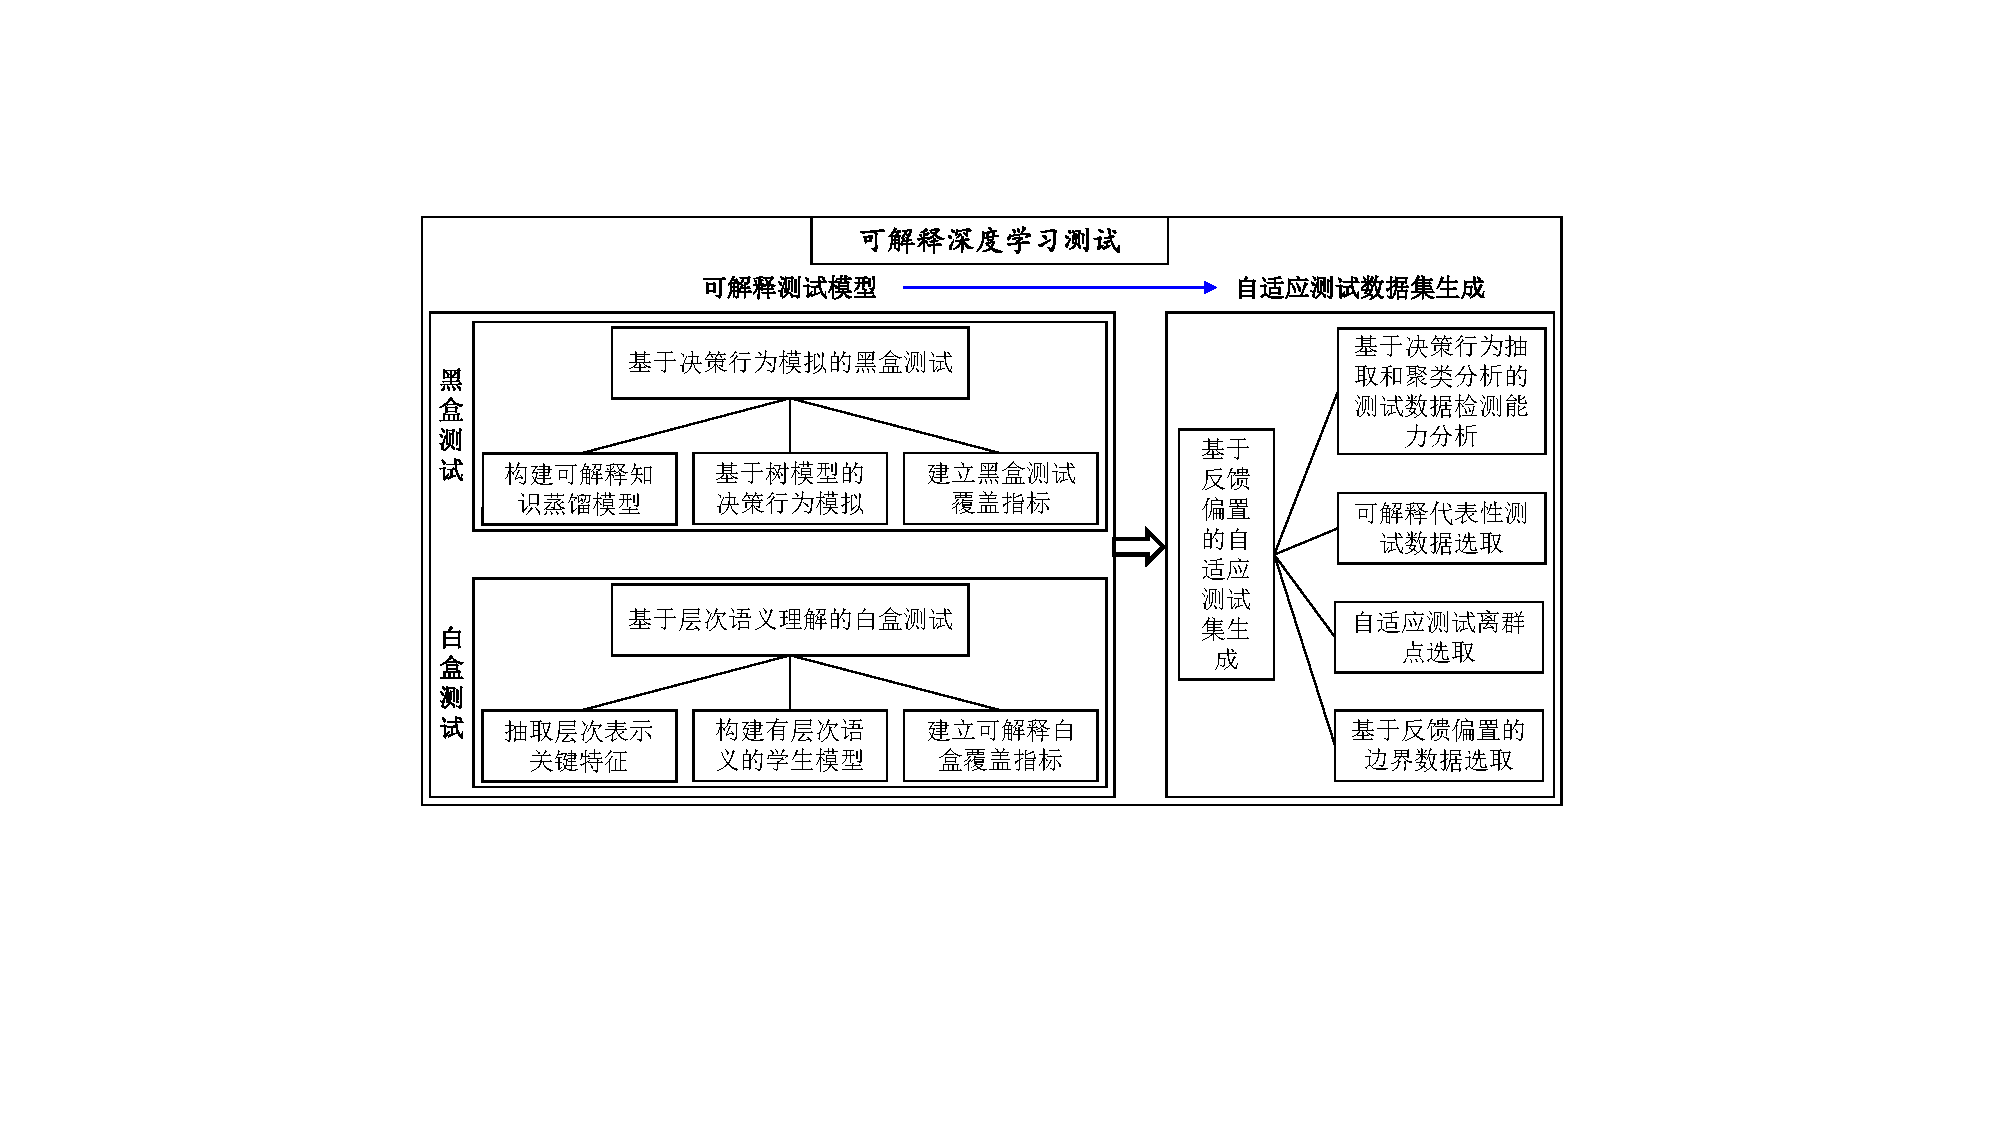
\includegraphics[width=0.95\textwidth]{ch3solution.pdf}
        \end{center}
        \caption{总体技术路线}
        \label{fig:ch3:solution}
    \end{small}
\end{figure}

围绕\ref{ch2target}制定的研究目标和\ref{ch2content}规划的研究内容,本项目拟定的
总体技术路线如\cref{fig:ch3:solution}所示。本项目针对大规模深度学习模型构建可解
释测试解决方案,从白盒测试和黑盒测试两个角度构建基于知识萃取的可解释测试方法,分
别提出基于层次语义理解的白盒测试覆盖指标和基于决策行为模拟的黑盒测试覆盖指标,并
在此基础上实现基于反馈偏置的自适应测试集生成,通过基于实例的解释方法和自适应反馈
偏置分别选取代表数据和边界数据,实现具有可解释性和伸缩性的深度学习模型测试框架。

\subsubsection{基于层次语义理解的白盒测试方法}\label{ch3_2}

本项目针对深度学习白盒测试的研究方案首先抽取具有语义逻辑的测试覆盖对象,在此基础
上构建具有可解释性的白盒测试覆盖指标。如\cref{fig:ch3:WBtestKD}所示,\textbf{首
先从给定的深度学习模型中抽取层次语义逻辑作为测试覆盖目标},具体而言,本项目拟采
线性判别分析(Linear Discriminative Analysis, LDA)抽取各层样本表示的关键特征,
同时利用降维效果提高测试大规模深度学习模型时的伸缩性。然后,利用自底向上的层次聚
类方法,对LDA得到的关键样本特征进行聚类,将具有相似判别决策能力的特征聚为一类。
本项目认为深度学习模型对输入的表示学习是一个从粗粒度到细粒度的过程,因此,浅层表
示(如第1组的输出)没有能力将样本分为最终指定的类别,仅能做到粗粒度分类,因此
\textbf{本项目拟修改层次聚类的优化目标,根据关键特征所在的层来决定层次聚类的类别
总数,以准确反映不同层级、不同粒度的决策语义}。

\begin{figure}[htp]
    \begin{small}
        \begin{center}
            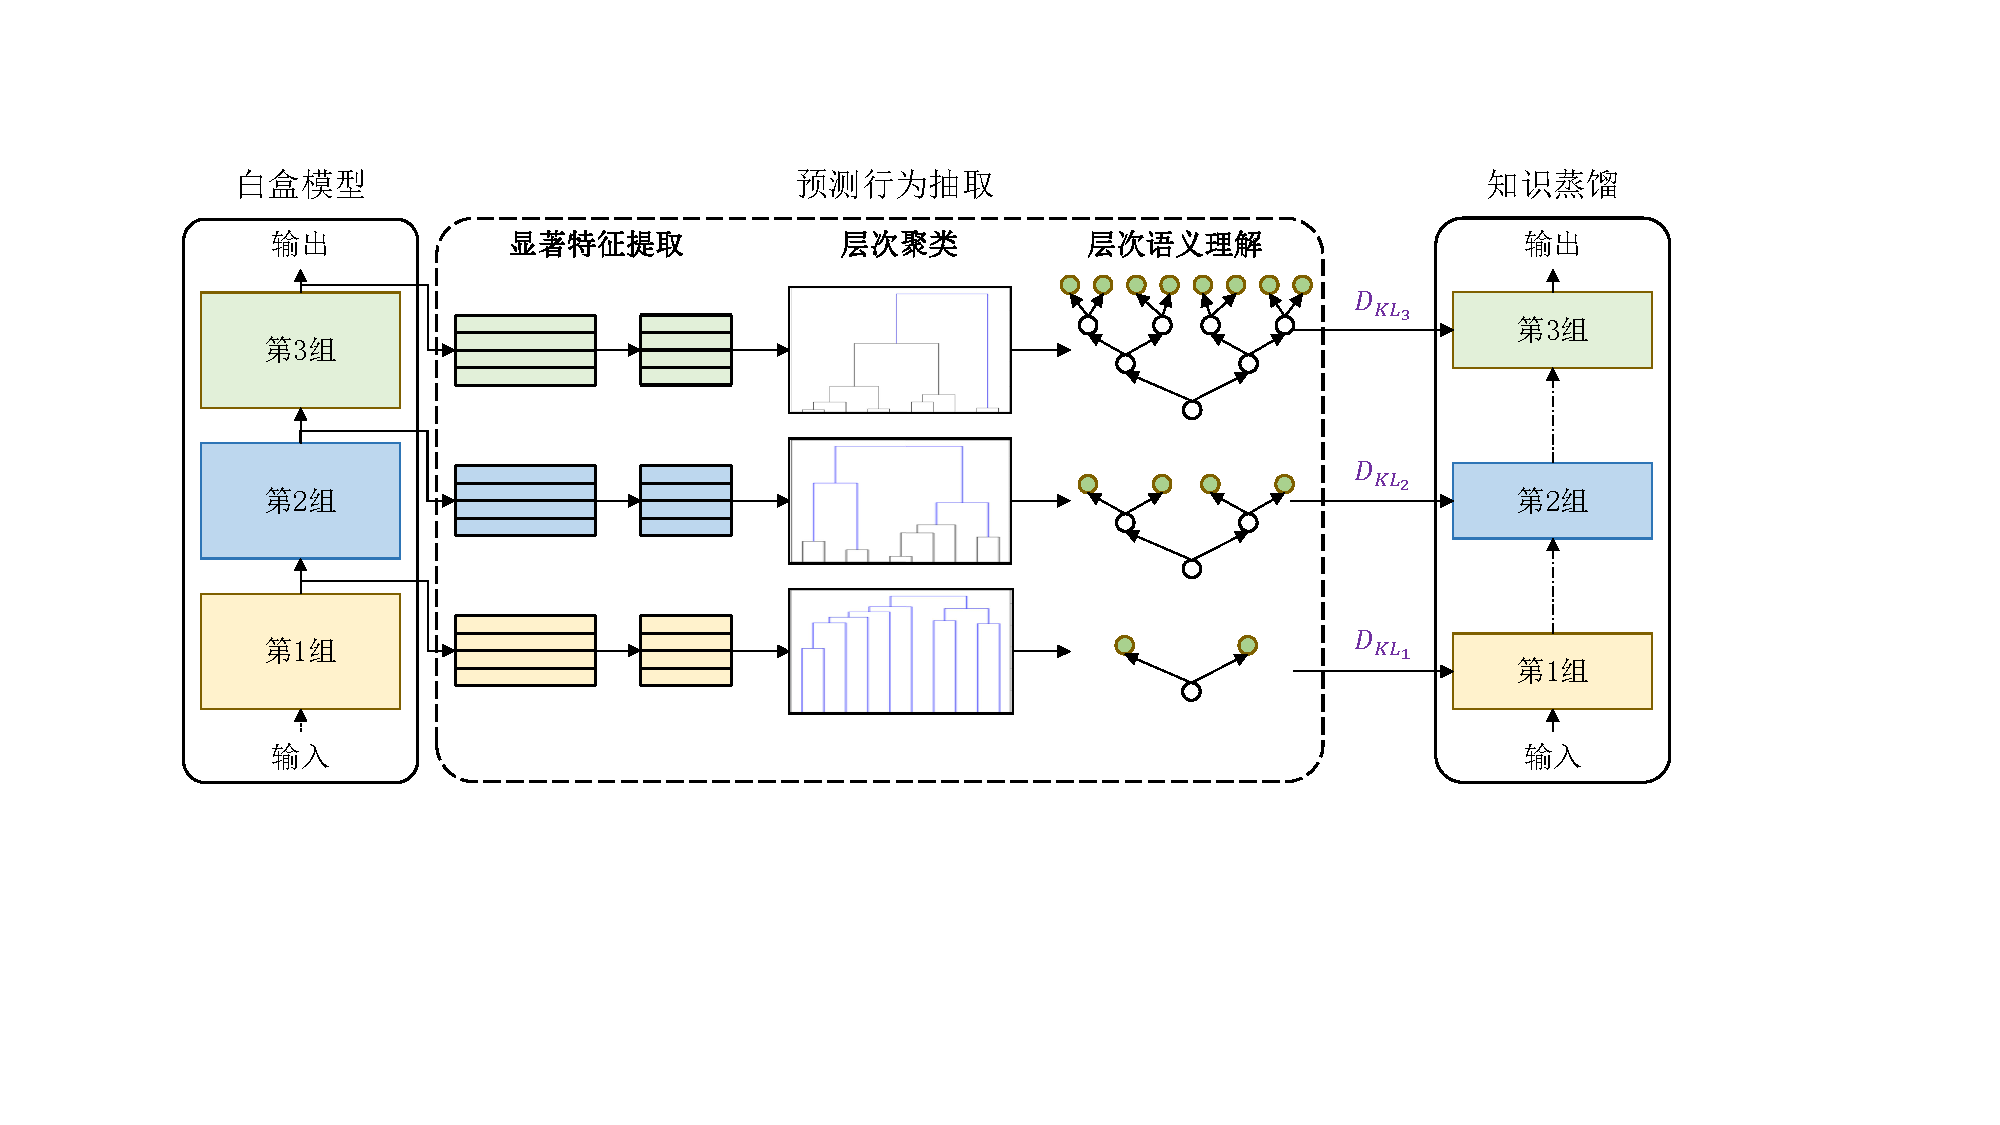
\includegraphics[width=0.95\textwidth]{ch3_WBtestKD.pdf}
        \end{center}
        \caption{基于层次语义理解的知识回顾研究方案}
        \label{fig:ch3:WBtestKD}
    \end{small}
\end{figure}

在得到各组(层)的决策语义后,本项目拟改进知识回顾的方式,\textbf{将各层
的决策语义融入“学生”模型的优化目标中},其主要思想如公式\eqref{eq:kd}所示:
\begin{equation}
    \mathcal{L} = \mathcal{L}_o + \beta\sum_{k=1}^L KL(p(f_s^k(\bm x_i)), p(g^k(y_i))) \,,
    \label{eq:kd}
\end{equation}
其中$\mathcal L_o$是学生模型原有的损失函数,$f_s^k(\bm x_i)$表示``学生''模型
第$k$层的表示向量,$g^k(y_i)$将数据标签$y_i$转换成第$k$层的语义标签,本项目拟用
KL散度来度量学生模型表示向量的分布是否和抽取的决策语义接近,作为损失函数的正
则项,引导学生模型训练。在得到可解释的学生模型后,本项目拟基于该模型提出
决策路径覆盖度测试指标。根据公式\eqref{eq:kd},在测试阶段,容易得到各层输出所属
的粗粒度类别,{如\cref{fig:ch3:WBtest}所示,本项目拟分析测试集对该决策路径图的覆
盖程度,用以评估测试用例集的充分性,同时,可检测学生模型针对某样本的分类过程
是否有异常决策路径(\cref{fig:ch3:WBtest}中红色虚线所示),以分析模型在边界数据
上的行为},具有异常决策路径的测试数据可能是引发模型错误的异常样本,\textbf{为测
试人员理解测试错误原因,辅助诊断和调试模型提供重要参考}。
\begin{figure}[htp]
    \begin{small}
        \begin{center}
            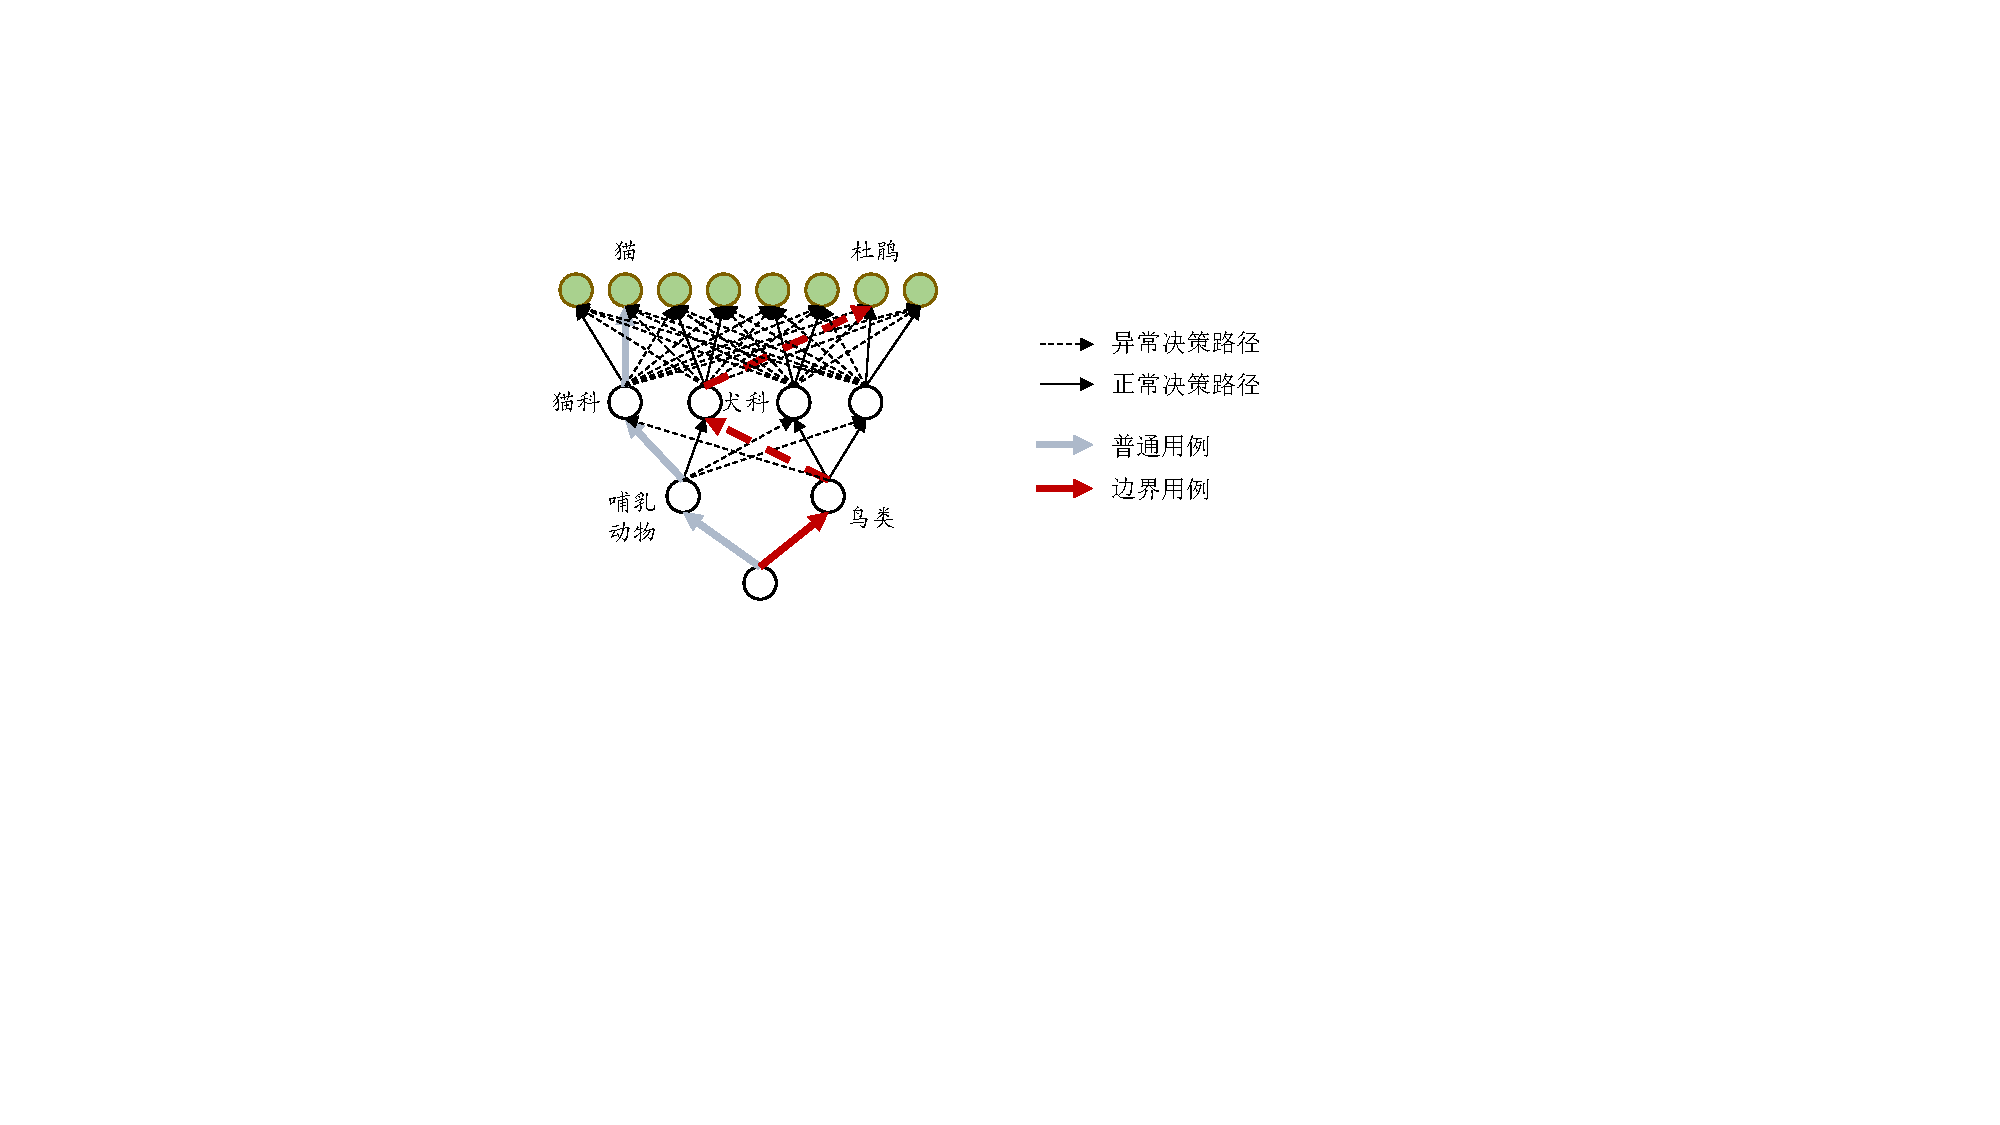
\includegraphics[width=0.65\textwidth]{ch3_WBtest.pdf}
        \end{center}
        \caption{基于可解释``学生''模型的覆盖度测试研究方案}
        \label{fig:ch3:WBtest}
    \end{small}
\end{figure}

\subsubsection{基于决策行为模拟的黑盒测试方法}\label{ch3_1}

借鉴传统软件的路径覆盖测试方法,许多研究提出针对深度学习模型的覆盖性测试方法(参
见\ref{relatedwork} 国内外研究现状及发展动态分析),这些测试覆盖指标和方法主要是
针对白盒的场景,即测试者掌握所有的训练数据和整个深度学习模型,但\textbf{在许多测试场
景中,测试者无法访问训练数据和模型内部结构,却仍需在部署前对模型进行测试},如深
度学习模型是某个公司私有的或者由第三方机构提供,他们只提供了接口或者打包的可执行
程序。因此,本项目面向黑盒测试场景,研究基于决策行为模拟的黑盒测试方法。

\cref{fig:ch3:2Btest}展示了本项目基于决策行为模拟的黑盒测试研究方法。如图所
示,本项目拟利用知识蒸馏技术萃取黑盒模型中的知识。\textbf{由于知识蒸馏可以完成
从教师模型到学生模型的知识迁移,因而学生模型可以看作是教师模型的全局近似,在一定
程度上反映了教师模型的整体逻辑,因此可以基于学生模型,提供对教师模型的全局解释}。
就申请人所知,目前尚未有基于知识蒸馏的深度学习覆盖测试研究工作。首先,本项目利用
知识蒸馏技术从黑盒模型(教师模型)中萃取知识,训练一个小模型(学生模型)模拟其预
测行为,在知识蒸馏中,教师模型被视为黑盒模型,正好契合本项目黑盒测试的场景。然
后,本项目拟设计针对小模型的测试方法,一方面,蒸馏得到的学生模型复杂度低,可有效
解决深度学习模型测试计算开销大的问题;另一方面,学生模型的内部结构可以自定义,测
试人员也可访问,本项目拟利用基于树的模型(如:决策树、随机森林等),以提高黑盒测
试结果的可解释性。

具体地,给定一个黑盒模型$\mathcal M$,本项目将$\mathcal M$视为教师模型,假定
对于任意的输入$x^{(i)}$,测试者仅能得到$\mathcal M$对于该输入预测的概率分布,即
$x^{(i)}$属于各类的概率,记为$p^{(i)}$。$(x^{(i)}, p^{(i)})$的对应关系即为模型
$\mathcal M$中蕴含的知识,将作为训练学生模型时的软目标。\textbf{本项目拟构建
基于树的模型作为学生模型,记为$\mathcal M_t$,以支持可解释模型测试}。根据知
识蒸馏的思想,在训练学生模型时,本项目融合软目标$(x^{(i)}, p^{(i)})$和硬目标
$(x^{(i)}, y^{(i)})$构建学生模型的损失函数,使树型模型的输出同时接近黑盒模型
的概率分布$p^{(i)}$和真实标签$y^{(i)}$。值得注意的是,在训练学生模型时,直接
使用教师模型SoftMax层的输出结果$p^{(i)}$不合适,因为小模型无法直接学习得到大
模型的效果,我们通过在学生模型的损失函数中引入知识蒸馏中的T(Temperature)参
数,放大分类错误的误差,缩小正确分类的误差,可有效提高学生模型训练的效果。

\begin{figure}[htp]
    \begin{small}
        \begin{center}
            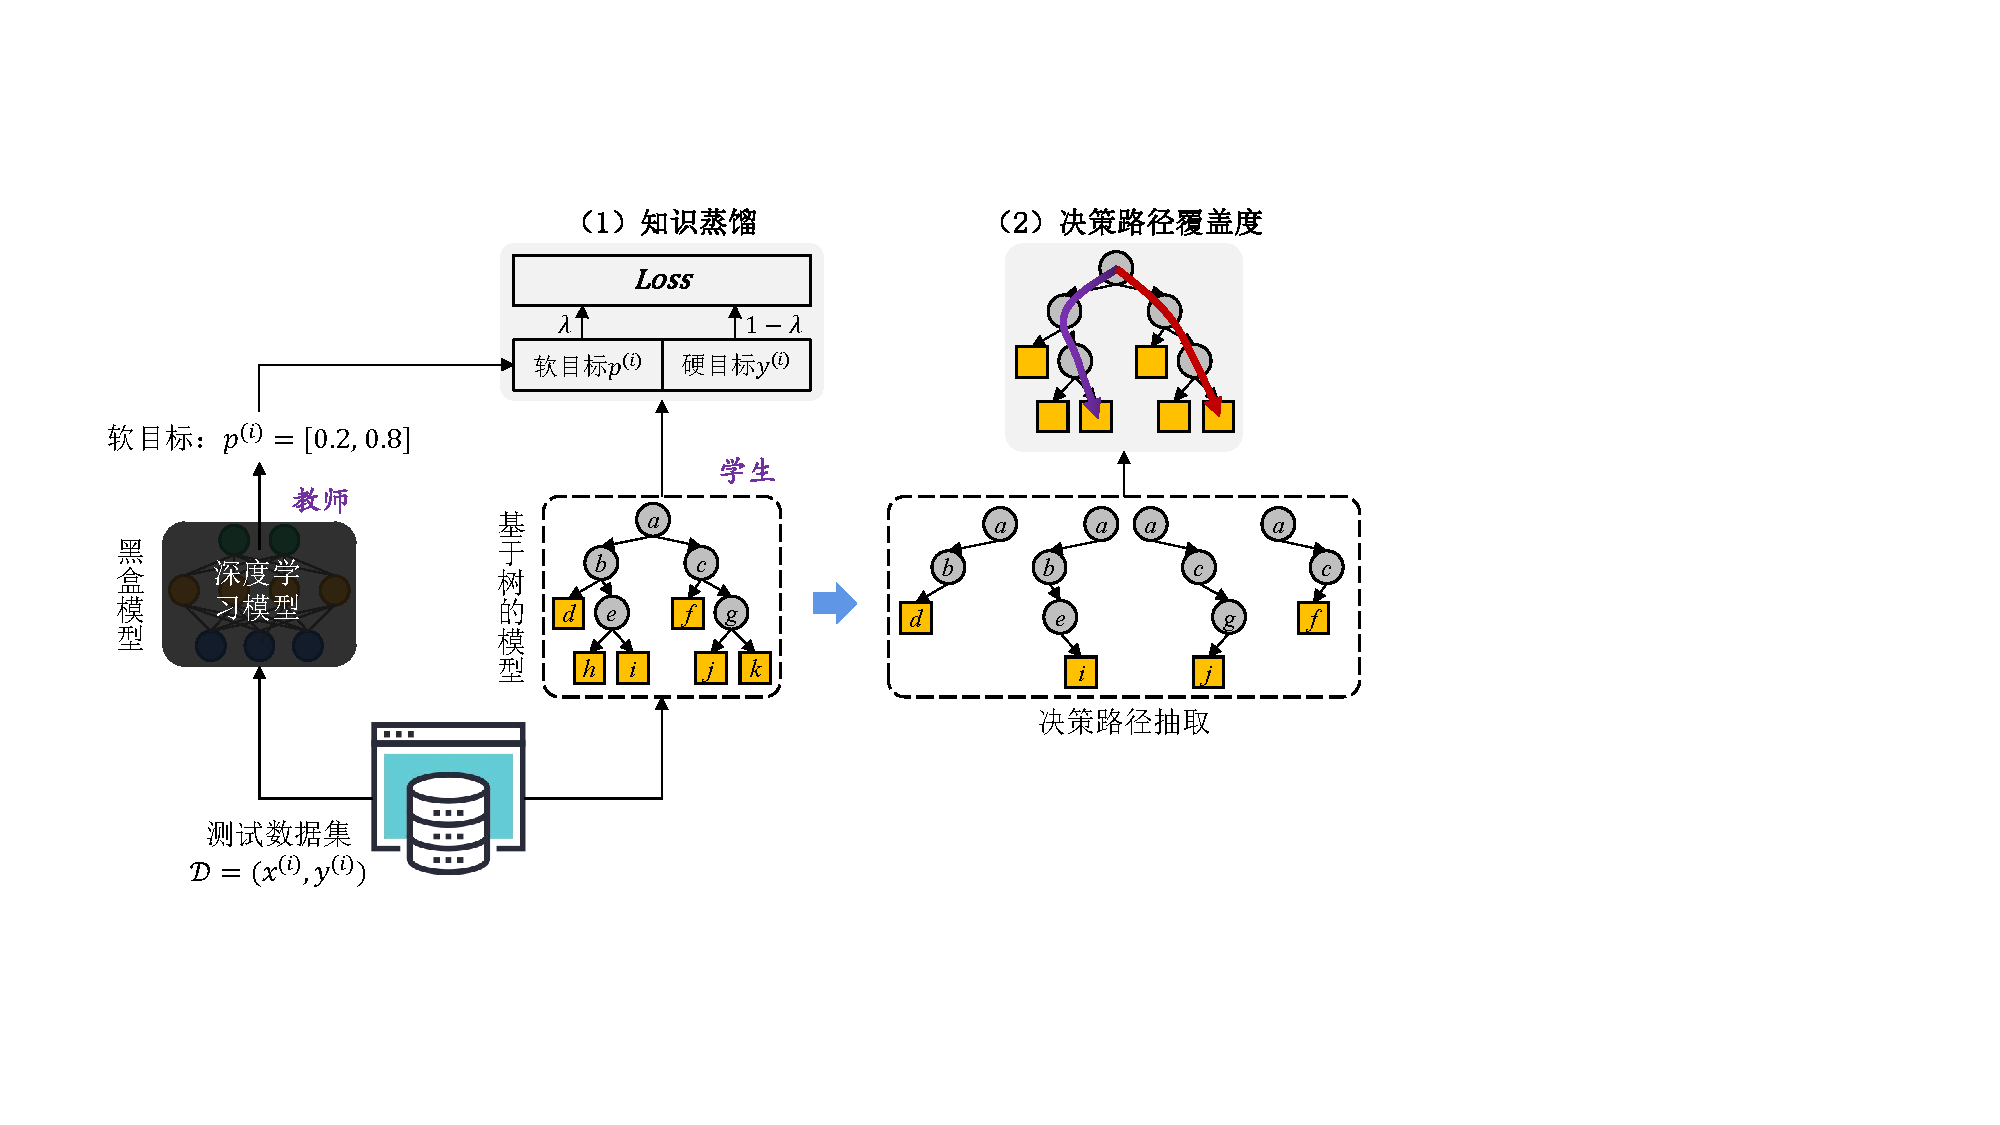
\includegraphics[width=0.9\textwidth]{ch3_2Btest.pdf}
        \end{center}
        \caption{基于决策行为模拟的黑盒测试研究方案}
        \label{fig:ch3:2Btest}
    \end{small}
\end{figure}


{本项目拟针对学生模型建立基于决策路径的覆盖性测试方法},知识蒸馏得到
的学生模型$\mathcal M_t$的预测行为非常接近原黑盒模型$\mathcal M$,针对
$\mathcal M_t$的覆盖度测试能比较准确地反映$\mathcal M$的泛化能力。首先,从基于树
的学生模型$\mathcal M_t$中抽取该模型对每个测试样本的决策路径,得到路径集合
$\mathcal P=\{t_1, t_2,\dots, t_l\}$,$l$表示路径数。然后,\textbf{利用
统计方法建立基于决策路径的覆盖度指标},以评估测试用例集的充分性,其基本思想为对
树模型的决策路径覆盖度高的测试用例集具有良好的充分性,在此基础上,本项目拟计算决
策路径覆盖频率和正态分布的拟合程度来评估测试用例集的分布,可采用
Kolmogorov-Smirnov检验、D检验等方法,并结合正太性检验方法的拟合优度和决策路径的
覆盖度作为测试用例集充分性评价指标。此外,\textbf{本项目拟利用树模型的可解释性,
总结归纳模型错误行为的原因,指导训练数据集扩充和模型优化}。



\subsubsection{基于反馈偏置的自适应测试集生成方法}\label{ch3_3}

为了平衡测试集的规模和质量,针对给定大规模无标注数据,本项目拟在有限标注成本空间
内生成具有高代表性和检测能力的测试集,采用\textbf{基于实例的解释(Example-based
Explanation)}思想,选取代表性的样本来解释模型结果,得到与大规模无标注数据具有近
似决策路径分布的测试子集,估算模型性能。同时,为对深度学习模型进行充分性测试,本
项目\textbf{融合自适应测试和测试反馈},不断从离群点中选取与已选测试数据距离最大
的离群点,并根据与预测错误的测试数据相似性,尽可能找到导致模型错误行为的测试数据
优先标注。

%\textbf{聚类分析和最大平均差异法}( Maximum Mean Discrepancy,MMD)选取与大规模
%无标注测试数据具有近似决策路径分布的代表性数据作为测试集,并反馈已选测试数据及
%其测试结果反馈,自适应选择测试数据。基于实例的方法主要是通过一些代表性的样本来
%解释聚类/分类结果的方法


\begin{figure}[htp]
    \begin{small}
        \begin{center}
            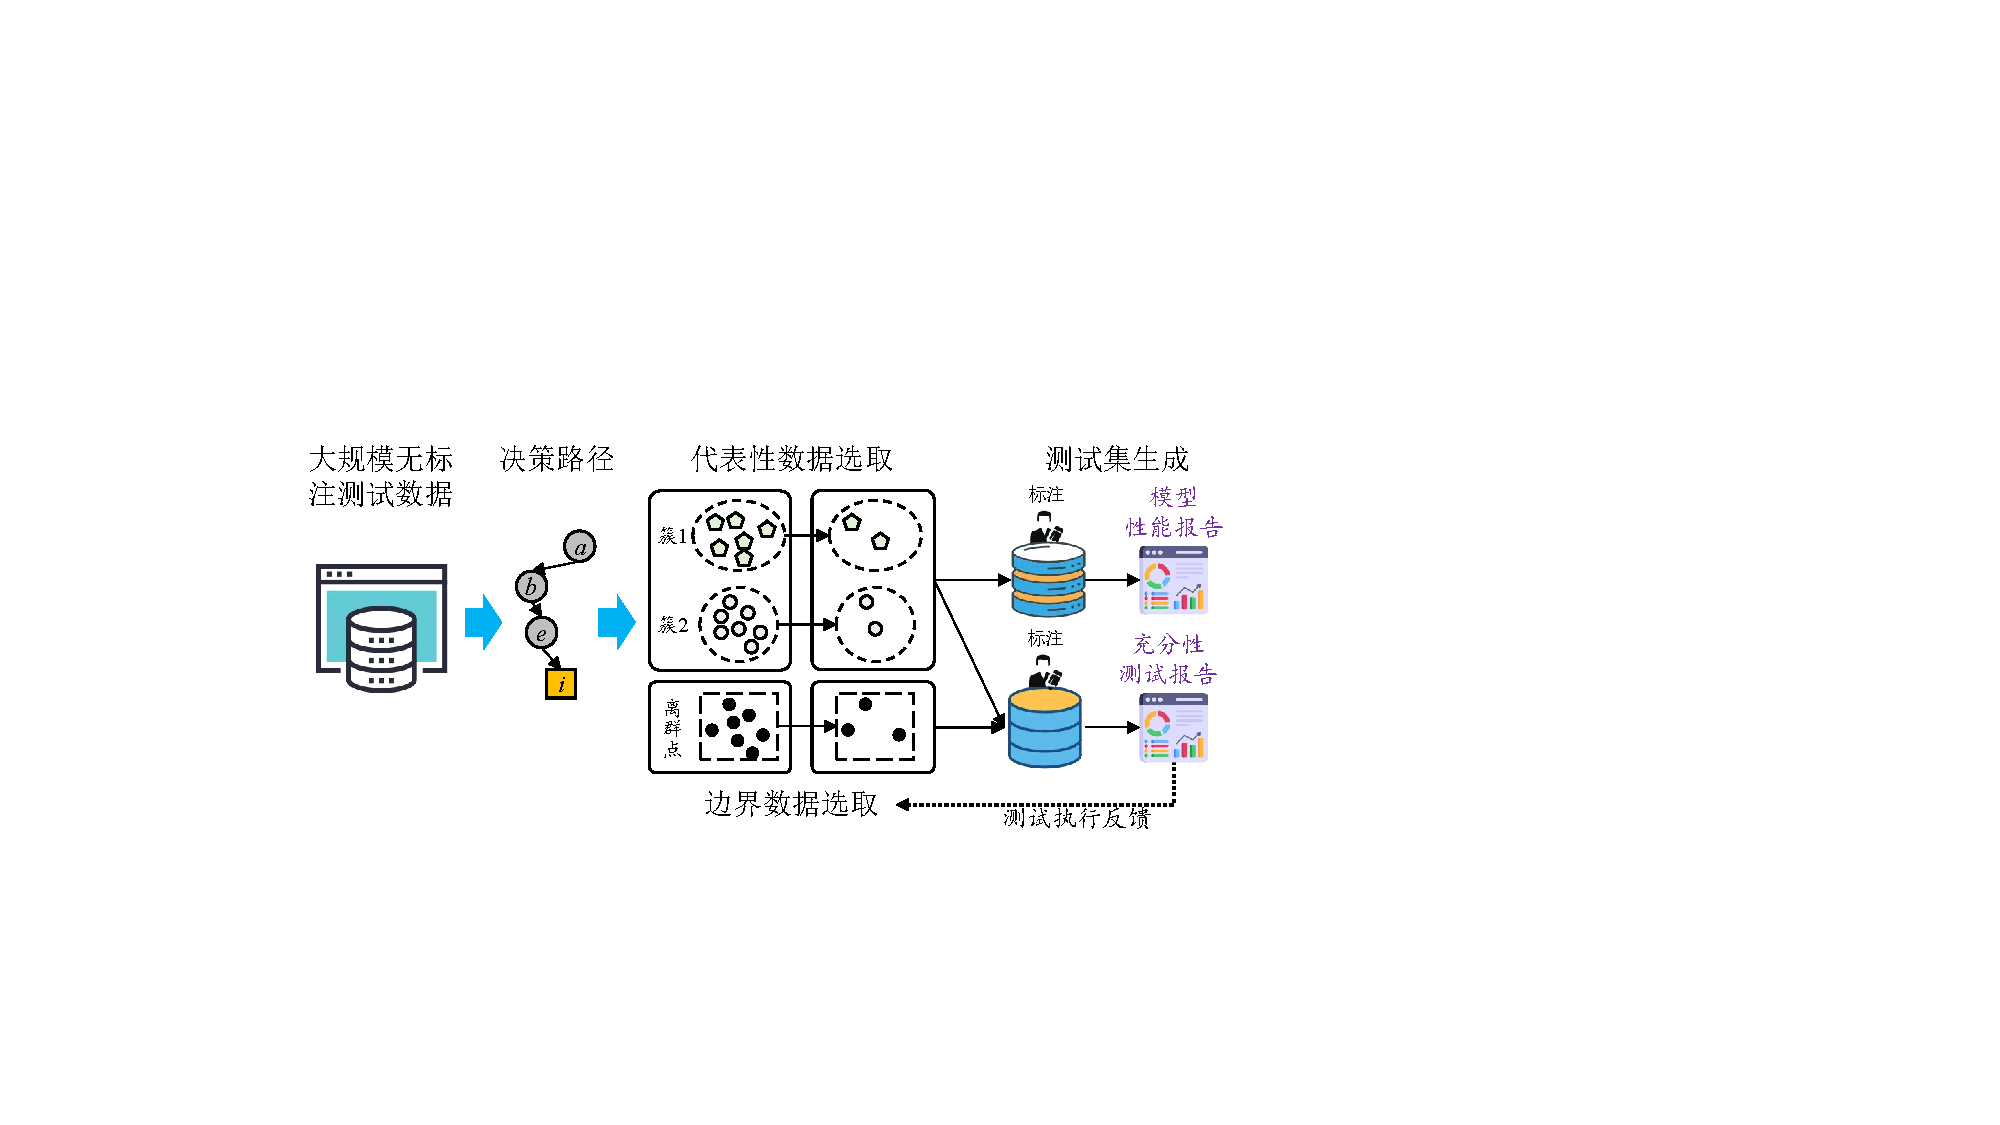
\includegraphics[width=0.85\textwidth]{ch3_TestSelection.pdf}
        \end{center}
        \caption{自适应测试集生成研究方案}
        \label{fig:ch3:interpretability}
    \end{small}
\end{figure}

\cref{fig:ch3:interpretability}是本项目针对深度学习模型自适应的测试集生成研究方
案示意图。为了提高可解释性和伸缩性,本项目在抽象可解释决策路径的基础上,结合决策
路径和聚类分析,区分具有不同检测能力的测试数据。以图中描述的模拟决策路径$t_i$为
例,每条决策路径对应的$n_i$个无标注测试数据为一组具有相似检测能力的测试数据。我
们对每组测试数据进行聚类分析,根据测试数据的规模大小将其聚为$k_i$类,将具有相同
决策路径的测试数据进一步划分为多簇。为了从大规模无标注数据中选取具有代表性的测试
数据,采用\textbf{最大平均差异算法}(Maximum Mean Discrepancy,MMD)从每类测试数
据中选取$m$个测试数据,若该类数少于$m$个则全部选取,构成初始测试子集。最大差异法
可表示为以下公式:
\begin{equation}
    \begin{aligned}
        \operatorname{MMD}(\mathcal{F}, P, Q)=\sup _{f \in \mathcal{F}}\left(\mathbb{E}_{X \sim P}[f(X)]-\mathbb{E}_{Y \sim Q}[f(Y)]\right)
    \end{aligned}
\end{equation}
其中$P$和$Q$分别为原测试数据分布和待选取测试数据分布,$\mathcal{F}$为再生西伯尔
空间,$\operatorname{MMD}(\mathcal{F}, P, Q)$用来衡量分布$P$和$Q$之间的距
离,\textbf{通过最小化MMD从每簇测试数据中选取具有解释性和代表性的测试数据,构成
代表性测试集},估算模型在大规模无标注数据上的性能。

为预防模型错误预测带来的损失,在测试覆盖指标和代表性测试集的基础上,进一步选择容
易导致错误行为的边界数据进行测试(见\cref{fig:ch3:interpretability})。在聚类分
析后,\textbf{采用自适应测试方法选取离群点,持续性选取与已选数据距离最大的测试数
据}进行充分性测试。同时,若经过标注和测试发现导致模型预测错误的测试数据,则
\textbf{将测试结果反馈到数据选择算子},选择与导致错误的测试数据具有相同决策路径
且在同簇中距离最近的测试数据进行充分性测试。

\subsection{可行性分析}

\textbf{(1)理论可行性:本项目技术路线中采用的思路方法已经在多个研究领域有所体
现}。例如技术路线中的知识蒸馏与知识回顾技术,是模型量化压缩领域非常重要的分支,
其核心是通过知识蒸馏完成知识迁移,训练对教师模型全局近似的学生模型,一方面能够对
教师模型进行量化压缩;另一方面,通过构建具有事前可解释性的学生模型能够提供对教师
模型的事后解释。本项目沿用知识蒸馏与知识回顾的思想,在不同测试场景下抽取具有语义
逻辑的测试覆盖对象,模拟模型的决策路径,并在此基础上结合统计方法,提出具有可解释
性的深度学习测试覆盖目标。知识蒸馏是模型量化和可解释性研究领域的热点之一,有较多
的成熟模型可以运用到本项目的场景中。因此,我们有理由相信,在针对深度学习模型的测
试领域,本项目提出和设计的一系列可解释性方案能够在构建可解释的测试方法上取得较好
的效果。

\textbf{(2)数据可行性:在本项目的前期相关工作中,项目申请人已经与工业界自动驾
驶领域相关单位进行了紧密的合作}。在基于深度学习模型的自动驾驶目标识别、转向(转
角)预测等任务上,申请人在测试数据集合和模型测试方法上都已经有足够的工作基础和能
力积累。而对于本项目最重要的测试报告数据而言,申请人已经与国汽智控(北京)科技有
限公司、中汽研(天津)汽车工程研究院等单位展开实质性合作,已经获取到了部分真实测
试数据和测试报告,并已经进行了部分报告的分析和总结。后期,申请人还将继续开展深入
的合作,获取更多的测试报告数据,结合公开数据集进行相应的补充和实验。

\textbf{(3)研究基础可行性:}本项目的申请人在

\subsubsection{技术可行性}

申请人前期调研了大量深度学习测试及其可解释性的研究工作(如\ref{relatedwork}节所
述),现有研究尚未形成可解释深度学习测试方法,主要受限于深度学习模型的规模太大、
可解释性差,而知识萃取方法可最大限度辅助模型理解,同时,最大平均差异法可以提供测
试数据选取的可解释性,因此,本项目利用知识萃取,构建基于路径的可解释覆盖测试指
标,并在此基础上,建立可解释数据选取方法,形成一套闭环深度学习测试框架,具有较强
的技术可行性。申请人之前的研究工作一直聚焦于深度学习测试和可解释性,在深度学习白
盒测试、模型可解释性和软件质量维护等方面已取得一定的研究成果,并在攻读博士期间主
导研发过开源工具。申请人所在项目组一直活跃在深度学习测试、软件安全、模型和数据安
全等相关领域,有着丰富的研究经验和技术积累。同时,在研究过程中,申请人与自动驾驶
公司(国汽智控)建立了合作关系,积累了大量可用于实验的真实数据集。因此,从技术上
说,本项目是可行的。

\iffalse
\subsubsection{团队合理性}

项目组在深度学习测试和模型安全具有一定的基础,积累了丰富的研究经验,在重要国际会
议上发表了多篇高水平论文,项目在开源软件开发和管理等方面也有丰富的积累,可为本项
目测试框架研发和开源推广提供保障。项目组梯队完善,队伍具有凝聚力和创造力,项目组
成员每周定期讨论,有着良好的科研氛围,同时对本项目的研究内容具有浓厚的研究兴趣。
申请人有着长期广泛的国内外合作者,申请人与合作导师Hua Ji教授,本学院的刘哲理教
授、范玲玲副教授,天津大学的陈森副教授等均有密切合作,他们一直活跃在软件测试、软
件安全和模型安全等领域的学术前沿,可为本项目提供技术指导。此外,申请人与联合培养
时的导师新加坡国立大学教授Siau-Cheng Kho一直保持密切联系,Kho教授长期从事软件安
全和深度学习方面的研究,是软件工程和软件安全方面非常活跃的科学家;申请人与新加坡
南洋理工大学教授Yang Liu合作密切,Liu教授在软件工程、开源软件分析域管理等方面有
着丰富且深入的研究,是相关领域的引领者。两位国际知名专家可为本项目提供技术指导。
\fi

\NsfcSection{4}{本项目的特色与创新之处;}{}

与现有研究工作相比,本项目的特色与创新之处体现在以下几方面:

\begin{itemize}
    \item[(1)] \textbf{针对黑盒测试中测试者无法访问模型内部结构的问题,本项目研
    究基于知识蒸馏的决策行为模拟方法,提高黑盒测试的有效性和可解释性}。目前针对
    深度学习黑盒测试的研究局限于模型无关的测试用例集多样性分析,缺乏对模型预测行
    为的建模,无法为模型开发提供有效的测试反馈信息;另一方面,仅分析测试用例集和
    模型的输入输出也难以针对模型构建可解释的测试覆盖指标。因此,在黑盒测试场景
    中,本项目利用知识蒸馏,从模型预测的概率分布出发,学习得到一个可解释``学生''
    模型,以模拟黑盒模型的决策行为,进而构建伸缩性强、可解释的覆盖测试指标,是本
    项目一大特色和创新之处。
    \item[(2)] \textbf{针对白盒测试中深度学习模型的可解释性差的问题,本项目研究
    基于层次语义理解的决策路径抽取方法,构建基于决策路径的覆盖性测试方法,提高白
    盒测试的伸缩性和可解释性}。现有白盒测试方法主要基于神经元取值和神经元覆盖度
    进行分析计算,由于深度学习模型包含较多神经元,现有方法计算复杂度高、缺乏可解
    释性,不具有实际应用价值。因此,在白盒测试场景中,本项目利用知识回顾的方法,
    分层抽取深度学习模型中的决策语义,并将抽取得到的多层语义信息融合到知识蒸馏
    中,进一步提高白盒测试的伸缩性,以适用于较大的深度学习模型。该研究可显著提高
    深度学习白盒测试的可解释性,是本项目相比于现有白盒测试方法的重要创新之处。
    \item[(3)] \textbf{针对测试数据选取和测试结果反馈缺乏可解释性的问题,本项目
    在路径覆盖指标的基础上,研究融合反馈偏置的自适应测试数据持续选取策略}。现有
    测试数据选取的研究缺乏可解释性,导致针对深度学习的有效测试信息较少,难以有效
    辅助开发人员修复模型缺陷。本项目在可解释黑盒测试和白盒测试的基础上,可以得到
    测试数据的决策路径分布,进而可根据决策路径分布和已测试样本的反馈偏置选取最具
    代表的测试数据,为测试人员提供全阶段的可解释测试方法,是本项目另一个重要的特
    色与创新之处。
\end{itemize}

\NsfcSection{5}{年度研究计划及预期研究结果}{(包括拟组织的重要学术交流活动、国际合作与交流计划等)。}

\subsection{年度研究计划}
本项目实施3年,具体年限为2023年1月1日至2025年12月31日。具体计划如下:

\textbf{第一阶段(2023年1月--2023年12月)},重点研究基于决策行为模拟的深度神经网
络黑盒测试方法,实现利用副本模型进行知识萃取的技术,并提出适用于复杂神经网络的测
试覆盖指标,具体包括:
\begin{itemize}[itemindent=2em]
    \item[(1)] 进行文献收集,整理,进而完善与细化研究方案。
    \item[(2)] 研究基于层次语义理解的测试覆盖目标抽取方法;
    \item[(3)] 提出适用于复杂神经网络的具有可解释性的测试覆盖指标;
    \item[(4)] 在国际期刊或会议上发表研究论文1-2篇,参加国际会议1-2次,并在会议上
          做论文成果报告,申请发明专利1项。
\end{itemize}

\textbf{第二阶段(2024年1月--2024年12月)},重点研究基于层次语义理解的深度神经网
络白盒测试技术,实现对原复杂模型的决策路径抽取和副本模型训练技术,并提出新的结构
覆盖指标,具体包括:
\begin{itemize}[itemindent=2em]
    \item[(1)] 研究对复杂模型的决策路径模拟方法;
    \item[(2)] 提出基于决策路径模拟的黑盒测试覆盖指标;
    \item[(3)] 本年度参加一次全国软件工程大会(NASAC 2024);
    \item[(4)] 在国际期刊或会议上发表研究论文1-2篇,参加国际会议1-2次,并在会议上做论文成果报告,申请发明专利1项。
\end{itemize}

\textbf{第三阶段(2025年1月--2025年12月)},重点研究基于反馈偏置的自适应测试集生
成方法,构建测试反馈机制,实现自适应的测试集生成方法,具体包括:
\begin{itemize}[itemindent=2em]
    \item[(1)] 研究利用基于实例的解释方法选取代表数据;
    \item[(2)] 研究融合反馈偏置的自适应方法选取边界数据;
    \item[(3)] 本年度邀请一次国内专家进行相关领域报告一次;
    \item[(4)] 在国际期刊或会议上发表研究论文1-2篇,参加国际会议1-2次,并在会议上
          做论文成果报告;
    \item[(5)] 项目总结,完成结项报告,准备验收。
\end{itemize}

\subsection{预期研究成果}

针对深度学习模型的可解释测试技术研究工作预期可以在构建可解释测试覆盖指标上取得以下研究成果:
\begin{itemize}[itemindent=2em]
    \item[(1)] 提出基于层次语义理解的测试覆盖目标抽取技术;
    \item[(2)] 构建具有层次语义逻辑的白盒测试覆盖指标;
    \item[(3)] 提出基于知识蒸馏的决策路径模拟技术;
    \item[(4)] 构建体现决策逻辑和决策依据的黑盒测试覆盖指标;
\end{itemize}

在可解释测试集生成上取得以下研究成果:
\begin{itemize}[itemindent=2em]
    \item[(1)] 提出基于可解释测试覆盖指标的测试数据生成技术;
    \item[(2)] 提出利用基于实例的解释方法选取代表数据的技术;
    \item[(3)] 构建反馈偏置机制,提出适用于边界测试数据选取的自适应测试方法;
    \item[(4)] 对提出的解释性方案效果通过基准数据集进行真实验证,并完成与相关工作的比较;
    \item[(5)] 构建完成面向基于人工智能的自动驾驶软件在转向/转角预测任务上的测试数据集、测试报告库。
\end{itemize}

本项目在完成深度学习模型的可解释测试技术研究的基础上,预计发表高水平学术论文3-6
篇,其中在CCF-A类推荐期刊/会议上发表学术论文3篇以上;完成一个面向深度学习模型的
可解释测试框架,并在基于深度学习的自动驾驶任务上进行真实验证;开源相关研究工作,
并提供说明和使用文档;申请专利2项;培养研究生2-3人。


%%%%%%%%%%%%%%%%%%%%%%%%%%%%%%%%%%%%%%%%%%%%%%%%%
\NsfcChapter{(二)研究基础与工作条件}{}


\NsfcSection{1}{研究基础}{(与本项目相关的研究工作积累和已取得的研究工作成绩);}
\iffalse
项目申请人蔡祥睿正在参与研究一项国家自然科学基金重点项目:{\kaishu{融合地理空间
的人物行为与事件演化(U1936206),2020年1月1日-2023年12月31日,项目负责人:袁晓
洁}}。该项目旨在地理空间数据和互联网数据,研究人物表示、群体识别、重大事件分析和
预测等问题,其中人物表示学习、融合时空特征的时间预测与本项目的患者表示学习、可解
释预测模型等研究问题相关,可为本项目提供研究思路。此外,该项目的实施经验可作为本
项目的参考,为本项目的顺利开展和完成提供帮助。
\fi

申请人蔡祥睿自攻读博士学位以来,{\kaishu 在国内外重要会议上发表学术论文15篇,其
中CCF A类会议4篇,CCF B类会议1篇}。此外,申请人在新加坡国立大学联合培养期间,曾
参与GEMINI(GEneralizable Medical Information aNalysis and Integration
Platform~\footnote{https://www.comp.nus.edu.sg/~dbsystem/gemini/})的研究与开
发,与新加坡国立大学医院(NUH)、新加坡国立大学医学组织(NUH),对电子医疗记录数
据分析和相关系统研发都有较丰富的积累。下面就申请人已发表、已投稿的研究工作和数据
集积累分别介绍与本项目相关的研究基础。

\subsection*{(1) 已发表研究工作}

针对医疗特征(概念)的表示学习,我们提出不同医疗特征具有不同的时间作用域范围,同
现有方法相比,我们的工作放宽了医疗特征的时间上下文范围,并在不同的时间段学习医疗
特征的影响力权重。实验表明,在考虑医疗特征的上述特点后,我们的方法能学到更好的特
征表示。该研究成果2018年发表于{\kaishu CCF推荐A类会议IJCAI}上。该论文虽然是针
对医疗特征表示的研究,但能够作为电子医疗记录输入的初始化向量,而且也为表现型表示
学习提供了思路,可作为本项目的研究基础和重要参考。

针对电子医疗记录缺失值插补的问题,我们在2018年最早提出将插补问题看作数据生成问
题,并首先利用GAN(Generative Adversarial Network)来实现缺失值的生成,该研究成
果于2018年发表于{\kaishu CCF推荐A类会议NeurIPS}。随后,鉴于原始GAN在本问题上训
练不稳定和效率低,我们又结合AutoEncoder和GAN提出端到端的缺失值插补方法,实现一次
训练,即可完成数据插补任务,该成果于2019年发表于{\kaishu CCF推荐A类会议
IJCAI}。基于GAN的研究工作为时序数据插补领域引进了新的生成式解决思路,这两个工作
可作为本项目电子医疗记录自动插补的研究基础,但它们没有考虑医疗偏差,也正是本项目
需要创新之处。

针对罕见单词的表示问题,我们提出了“单词-子单词”层次表示模型,在子单词表示学习的
基础上,组合转换得到单词表示的方法,并首次研究子单词向量维度对单词表示的影响,该
研究成果发表于2019年发表于{\kaishu CCF推荐B类会议DASFAA},单词拆分本质上思路和本
项目的患者表示拆分为表现型向量是一致的,虽然该研究工作与本项目不直接相关,但其研
究思路可作为本项目的借鉴。

\subsection*{(2) 已投稿研究工作}

针对融合医学偏差的EMR插补问题,我们提出了基于缺失标记矩阵的注意力机制,并将缺失
标记矩阵的信息传入针对观察到的数据所建的模型中,实验证明,在多个电子医疗记录上,
该方法明显优于现有模型。该工作已投稿于{\kaishu CCF推荐A类会议IJCAI},并已于2019
年11月{\kaishu 申请国家发明专利}(电子医疗记录数据的缺失值填充方法,
201911210250.7),该工作可作为本项目针对EMR插补问题构建对偶模型的直接研究基础。

针对医学领域标记样本较少的问题,我们已经在眼底影像数据上开展过研究,通过领域自适
应的方法,可以是模型学习到泛化性更好的数据表示,不仅在未标注的数据集上取得较好效
果,也能提高标注数据集的分类效果,该工作已投稿{\kaishu SCI一区期刊IEEE
Transaction on Medical Imaging}。该研究的成功表明,本项目在队列识别中所面临的弱
监督学习可借鉴领域自适应的思想。

\subsection*{(3) 项目经验和数据集积累}

申请人在新加坡国立大学联合培养期间,曾参与GEMINI(GEneralizable Medical
Information aNalysis and Integration
Platform~\footnote{https://www.comp.nus.edu.sg/~dbsystem/gemini/})的研究与开
发,该项目旨在构建通用的医疗数据集成和分析平台,{\kaishu 申请人在项目中负责研
发医学概念嵌入预处理模块,参与工作空间和数据集管理开发,实现ICU死亡预测、糖尿病
进展建模和X-Ray影像分析等临床应用模块}。申请人积累了大量电子医疗记录分析的经验,
也发现电子医疗记录分析存在巨大的挑战,即本申请书提出的挑战和研究内容。此外,
{\kaishu 申请人积累了多个研究数据集,如MIMIC-III, ADNI, Parkinson等}。此外,
{\kaishu 申请人参与“南开大学-基准联合医学研究中心”建设},已积累来自广州15家医
院的肺癌患者的电子医疗记录;通过和北京大学医疗健康大数据国家研究院合作,积累DKD
慢性肾病患者队列数据,包含约3000个患者。这些项目经验和数据积累是本项目重要的研究
基础。

基于上述工作,申请人有信心达到本项目的研究目标,并取得高水平研究成果。

\NsfcSection{2}{工作条件}{(包括已具备的实验条件,尚缺少的实验条件和拟解决的途径,包括利用国家实验室、国家重点实验室和部门重点实验室等研究基地的计划与落实情况);}

项目依托南开大学数据库与信息系统实验室,本实验室通过前期研究课题的积累,已经建有
大数据计算集群,拥有10余个GPU计算节点、服务器20余台和微机100余台,其中包含IBM、
DELL等品牌高性能服务器,并安装了较齐全的软件系统以及开发工具,添置了比较齐备的网
络设备,配置了Hadoop和Spark云计算平台,该平台以万兆带宽连接到学校的数据中心,通
过校园网与Internet网连接,其强大的计算能力和I/O能力为本项目提供了测试平台和非常
有利的条件。它可作为我们开展研究工作的场所,所以完成本项目研究的实验条件已基本具
备。实验室每周举行组会,探讨学科前沿科学问题,进行头脑风暴,激发研究热情和创新
点。实验室每两周举行一次大组会,总结当前工作,制定新的规划,保证研究方向和技术路
线正确。实验室积极严谨的科研氛围是保证本项目实施的重要因素。

申请人参与建设“南开大学-基准联合医学研究中心”,该平台由南开大学计算机学院和广州
基准医疗有限责任公司联合共建,旨在面向多模态医学数据,利用人工智能技术实现高发癌
症的早诊早筛,广州基准公司提供数据和生物信息学专家支持,目前申请人所带领的团队已
在肺癌筛查方面取得了一定的突破。在该平台的支持下,申请人及研究团队已与天津市肿瘤
医院肺癌专科建立合作。此外,申请人与北京大学医疗健康大数据国家研究院张路霞教授团
队合作研究慢性肾病患者病情进展预测。这些医疗机构和单位可为本项目提供数据支持和医
学专家指导,保证本项目的顺利完成。

综上所述,本项目的软硬件条件都已具备,尚无缺少的实验条件。

\NsfcSection{3}{正在承担的与本项目相关的科研项目情况}{(申请人正在承担的与本项目相关的科研项目情况,包括国家自然科学基金的项目和国家其他科技计划项目,要注明项目的资助机构、项目类别、批准号、项目名称、获资助金额、起止年月、与本项目的关系及负责的内容等);}

无

\NsfcSection{4}{完成国家自然科学基金项目情况}{(对申请人负责的前一个已资助期满的科学基金项目(项目名称及批准号)完成情况、后续研究进展及与本申请项目的关系加以详细说明。另附该项目的研究工作总结摘要(限500字)和相关成果详细目录)。}

%%%%%%%%%%%%%%%%%%%%%%%%%%%%%%%%%%%%%%%%%%%%%%%%%

无

\NsfcChapter{(三)其他需要说明的问题}{}

\NsfcSection{1}{}{申请人同年申请不同类型的国家自然科学基金项目情况(列明同年申请的其他项目的项目类型、项目名称信息,并说明与本项目之间的区别与联系)。}

无

\NsfcSection{2}{}{具有高级专业技术职务(职称)的申请人是否存在同年申请或者参与申请国家自然科学基金项目的单位不一致的情况;如存在上述情况,列明所涉及人员的姓名,申请或参与申请的其他项目的项目类型、项目名称、单位名称、上述人员在该项目中是申请人还是参与者,并说明单位不一致原因。}

无

\NsfcSection{3}{}{具有高级专业技术职务(职称)的申请人是否存在与正在承担的国家自然科学基金项目的单位不一致的情况;如存在上述情况,列明所涉及人员的姓名,正在承担项目的批准号、项目类型、项目名称、单位名称、起止年月,并说明单位不一致原因。}

无

\NsfcSection{4}{}{其他。}

无


\end{document}
